%%%%%%%%%%%%%%
%% Run LaTeX on this file several times to get Table of Contents,
%% cross-references, and citations.

%% If you have font problems, you may edit the w-bookps.sty file
%% to customize the font names to match those on your system.

%% w-bksamp.tex. Current Version: Feb 16, 2012
%%%%%%%%%%%%%%%%%%%%%%%%%%%%%%%%%%%%%%%%%%%%%%%%%%%%%%%%%%%%%%%%
%
%  Sample file for
%  Wiley Book Style, Design No.: SD 001B, 7x10
%  Wiley Book Style, Design No.: SD 004B, 6x9
%
%
%  Prepared by Amy Hendrickson, TeXnology Inc.
%  http://www.texnology.com
%%%%%%%%%%%%%%%%%%%%%%%%%%%%%%%%%%%%%%%%%%%%%%%%%%%%%%%%%%%%%%%%

%%%%%%%%%%%%%
% 7x10
%\documentclass{wileySev}

% 6x9
\documentclass{wileySix}

\usepackage{graphicx}

%%%%%%%
%% for times math: However, this package disables bold math (!)
%% \mathbf{x} will still work, but you will not have bold math
%% in section heads or chapter titles. If you don't use math
%% in those environments, mathptmx might be a good choice.

% \usepackage{mathptmx}

% For PostScript text
\usepackage{w-bookps}

%%%%%%%%%%%%%%%%%%%%%%%%%%%%%%%%%%%%%%%%%%%%%%%%%%%%%%%%%%%%%%%%
%% Other packages you might want to use:

% for chapter bibliography made with BibTeX
% \usepackage{chapterbib}

% for multiple indices
% \usepackage{multind}

% for answers to problems
% \usepackage{answers}

%%%%%%%%%%%%%%%%%%%%%%%%%%%%%%
%% Change options here if you want:
%%
%% How many levels of section head would you like numbered?
%% 0= no section numbers, 1= section, 2= subsection, 3= subsubsection
%%==>>
\setcounter{secnumdepth}{3}

%% How many levels of section head would you like to appear in the
%% Table of Contents?
%% 0= chapter titles, 1= section titles, 2= subsection titles, 
%% 3= subsubsection titles.
%%==>>
\setcounter{tocdepth}{2}

%% Cropmarks? good for final page makeup
%% \docropmarks

%%%%%%%%%%%%%%%%%%%%%%%%%%%%%%
%
% DRAFT
%
% Uncomment to get double spacing between lines, current date and time
% printed at bottom of page.
% \draft
% (If you want to keep tables from becoming double spaced also uncomment
% this):
% \renewcommand{\arraystretch}{0.6}
%%%%%%%%%%%%%%%%%%%%%%%%%%%%%%

%%%%%%% Demo of section head containing sample macro:
%% To get a macro to expand correctly in a section head, with upper and
%% lower case math, put the definition and set the box 
%% before \begin{document}, so that when it appears in the 
%% table of contents it will also work:

\newcommand{\VT}[1]{\ensuremath{{V_{T#1}}}}

%% use a box to expand the macro before we put it into the section head:

\newbox\sectsavebox
\setbox\sectsavebox=\hbox{\boldmath\VT{xyz}}

%%%%%%%%%%%%%%%%% End Demo


\begin{document}


\booktitle{Survey Methodology}
\subtitle{This is the Subtitle}

\authors{Robert M. Groves\\
\affil{Universitat de les Illes Balears}
Floyd J. Fowler, Jr.\\
\affil{University of New Mexico}
}

\offprintinfo{Survey Methodology, Second Edition}{Robert M. Groves}

%% Can use \\ if title, and edition are too wide, ie,
%% \offprintinfo{Survey Methodology,\\ Second Edition}{Robert M. Groves}

%%%%%%%%%%%%%%%%%%%%%%%%%%%%%%
%% 
\halftitlepage

\titlepage


\begin{copyrightpage}{2007}
Survey Methodology / Robert M. Groves . . . [et al.].
\       p. cm.---(Wiley series in survey methodology)
\    ``Wiley-Interscience."
\    Includes bibliographical references and index.
\    ISBN 0-471-48348-6 (pbk.)
\    1. Surveys---Methodology.  2. Social 
\  sciences---Research---Statistical methods.  I. Groves, Robert M.  II. %
Series.\\

HA31.2.S873 2007
001.4'33---dc22                                             2004044064
\end{copyrightpage}

\dedication{To my parents}

\begin{contributors}
\name{Masayki Abe,} Fujitsu Laboratories Ltd., Fujitsu Limited, Atsugi,
Japan

\name{L. A. Akers,} Center for Solid State Electronics Research, Arizona
State University, Tempe, Arizona

\name{G. H. Bernstein,} Department of Electrical and
Computer Engineering, University of Notre Dame, Notre Dame, South Bend, 
Indiana; formerly of
Center for Solid State Electronics Research, Arizona
State University, Tempe, Arizona 
\end{contributors}

\contentsinbrief
\tableofcontents
\listoffigures
\listoftables


\begin{foreword}
This is the foreword to the book.
\end{foreword}

\begin{preface}
This is an example preface.
This is an example preface.
This is an example preface.
This is an example preface.

\prefaceauthor{R. K. Watts}
\where{Durham, North Carolina\\
September, 2007}

\end{preface}


\begin{acknowledgments}
From Dr.~Jay Young, consultant from Silver Spring, Maryland, I received
the initial push to even consider writing this book. Jay was a constant
``peer reader'' and very welcome advisor durying this year-long process.


To all these wonderful people I owe a deep sense of gratitude especially now
that this project has been completed.
\authorinitials{G. T. S.}
\end{acknowledgments}

\begin{acronyms}
\acro{ACGIH}{American Conference of Governmental Industrial Hygienists}
\acro{AEC}{Atomic Energy Commission}
\acro{OSHA}{Occupational Health and Safety Commission}
\acro{SAMA}{Scientific Apparatus Makers Association}
\end{acronyms}

\begin{glossary}
\term{NormGibbs}Draw a sample from a posterior distribution
of data with an unknown mean and variance using Gibbs sampling.

\term{pNull}Test a one sided hypothesis from a numberically
specified posterior CDF or from a sample from the posterior

\term{sintegral}A numerical integration using Simpson's rule
\end{glossary}

\begin{symbols}
\term{A}Amplitude

\term{\hbox{\&}}Propositional logic symbol 

\term{a}Filter Coefficient

\bigskip

\term{\mathcal{B}}Number of Beats
\end{symbols}

\begin{introduction}

%% optional, but if you want to list author:

\introauthor{Catherine Clark, PhD.}
{Harvard School of Public Health\\
Boston, MA, USA}

The era of modern \index{microelectronics}\index{microelectronics!modern} 
began in 1958 with the invention of the
integrated circuit by J.~S.~Kilby
 of Texas Instruments \cite{kilby}.
His first chip is shown in Fig.~I. For comparison,
Fig.~I.2 shows a modern microprocessor chip, \cite{beren}.


This is the introduction.
This is the introduction.
This is the introduction.
This is the introduction.
This is the introduction.
This is the introduction.

\begin{equation}
ABC {\cal DEF} \alpha\beta\Gamma\Delta\sum^{abc}_{def}
\end{equation}


\begin{chapreferences}{3.}
\bibitem{zkilby}J. S. Kilby,
``Invention of the Integrated Circuit,'' {\it IEEE Trans. Electron Devices,}
{\bf ED-23,} 648 (1976).

\bibitem{zhamming}R. W. Hamming,
                 {\it Numerical Methods for Scientists and 
                 Engineers}, Chapter N-1, McGraw-Hill, 
                 New York, 1962.

\bibitem{zHu}J. Lee, K. Mayaram, and C. Hu, ``A Theoretical
               Study of Gate/Drain Offset in LDD MOSFETs''
                     {\it IEEE Electron Device Lett.,} {\bf EDL-7}(3). 152 
                     (1986).
\end{chapreferences}
\end{introduction}


\part[Submicron Semiconductor Manufacture]
{Submicron Semiconductor\\ Manufacture}

\chapter{Home}

\chapter{Overview}

\chapter{Environtment Setup}

\chapter{Basic Syntax}

\chapter{Variabel Type}

\chapter{Basic Operator}

\chapter{Desicion Making}

\chapter{Loop}

\chapter{Numbers}

\chapter{Strings}

\chapter{Lists}

\chapter{Tuples}

\chapter{Dictionary}

\chapter{Functions}

\chapter{Modules}

\chapter{Files I/O}

\chapter{Exceptions}

\chapter{Clasess/Object}

\chapter{Reg Expression}

\chapter{Networking}

\chapter{CGI Programming}
\section{Common Gateway Interface}
\subsection{Sejarah Common Gateway Interface}
Pada tahun 1993, tim National Center for Supercomputing Applications (NCSA) menulis spesifikasi untuk memanggil executable command line di milis www-talk. [2] [3] [4] Pengembang server Web lainnya menggunakannya, dan telah menjadi standar untuk server Web sejak saat itu. Sebuah kelompok kerja yang dipimpin oleh Ken Coar dimulai pada bulan November 1997 untuk mendapatkan definisi NCSA tentang CGI yang lebih formal. [5] Karya ini menghasilkan RFC 3875, yang menentukan Versi CGI 1.1. Secara khusus disebutkan di RFC adalah kontributor berikut: [6]
\begin{itemize}
\item Rob McCool (penulis Server Web HTTP NCSA)
\item John Franks (penulis GN Web Server)
\item Ari Luotonen (pengembang CERN httpd Web Server)
\item Tony Sanders (penulis Web Server Plexus)
\item George Phillips (pengelola server Web di University of British Columbia)
\end{itemize}
Secara historis skrip CGI sering ditulis menggunakan bahasa C. RFC 3875 "Common Gateway Interface (CGI)" secara parsial mendefinisikan CGI menggunakan C, [7] seperti dalam mengatakan bahwa variabel lingkungan ``diakses oleh perpustakaan perpustakaan umum getenv () atau variabel lingkungan``.  \cite{mccool1993common}
\subsection{Common Gateway Interface}
Common Gateway Interface atau disingkat CGI merupakan standar untuk menghubungkan berbagai program aplikasi ke halaman web. CGI mirip dengan program komputer yang menjadi perantara antara standar HTML yang menjadikan tampilan web dengan program lain, seperti basis data (database). Hasil yang diperoleh dari proses pencarian dikirimkan kembali ke halaman web untuk ditampilkan dalam format HTML. CGI (Common Gateway Interface) adalah bentuk dari hubungan interaktif di mana client (browser) bisa mengirimkan suatu masukan kepada server, dan server mengolah masukan tersebut serta mengembalikannya kepada client (browser). Contoh sederhana adalah saat kita menggunakan sebuah mesin pencari. Saat kita menuliskan keyword dan menekan tombol Search maka browser akan mengirimkan keyword tersebut ke server. Keyword tersebut lalu diolah oleh server dan server mengirimkan data hasil pengolahan (yang sesuai dengan keyword yang kita masukkan) ke browser kita. Jadi yang akan kita lihat pada browser adalah  hanya data yang sesuai dengan keyword yang kita masukkan. 
Untuk dapat menggunakan CGI syarat yang utama adalah server dengan sistem operasi UNIX (beserta variantnya). Namun perlu kita perhatikan bahwa tidak semua server UNIX (gratis) mampu menangani dan melayani CGI. Server-server yang melayani penempatan web yang berlayanan gratis seperti Geocities dan Homepage, tidak akan mengijinkan penggunaan script CGI dalam web kita. Untuk itu kita bisa mencoba Virtual Avenue, Tripod, atau Hypermart.
	Program CGI ditulis dengan menggunakan bahasa yang dapat dimengerti oleh sistem misalnya C/C++, Fortran, Perl, Tcl, Visual Basic, dan lain-lain. Pemilihan bahasa yang digunakan tergantung dari sistem yang digunakan. Jika bahasa pemrograman yang digunakan seperti C atau Fortran maka program-program yang kita buat harus dikompile terlebih dahulu sebelum dijalankan sehingga pada server akan terdapat source code dan program hasil kompilasi. Berbeda jika bahasa yang digunakan yaitu bahasa script seperti PERL, TCL, atau Unix Shell maka hanya akan terdapat script itu sendiri (tanpa ada source code). Jika dibandingkan saat ini banyak orang yang lebih memilih untuk menggunakan sebuah script CGI daripada menggunakan bahasa pemrograman karena lebih mudah untuk di-compile dan dimodifikasi.  
	Pada awalnya CGI merupakan~salah satu yang mendekati aplikasi server-side programming.  Program CGI yang paling sering digunakan yaitu~C++ dan perl.  CGI merupakan bagian dari web server yang dapat berkomunikasi dengan program lain yang ada di server. Dengan CGI web server dapat memanggil program yang dibuat dari berbagai bahasa pemrograman (Common). Interaksi antara pengguna dengan berbagai aplikasi, misalnya database, dapat dijembatani oleh CGI (Gateway). 
	CGI (Common Gateway Interface) merupakan skrip tertua dalam bidang pemrograman web. Skrip bisa didefinisikan sebagai rangkaian dari beberapa instruksi program. Untuk membuat skrip yang dapat dijalankan pada web diperlukan pengetahuan pemograman. 
	CGI sendiri telah muncul sejak teknologi web diperkenalkan di dunia pada awal tahun 1990, bersama dengan kemunculan CERN, web server pertama di dunia. CGI disediakan sebagai tool atau perlengkapan untuk membuat program web. CGI digunakan untuk membuat program-program tampilan web yang lebih interaktif, koneksi ke basis data, bahkan membuat permainan (game). 
	CGI pada masa-masa awalnya dibuat dengan bahasa C, bahasa yang juga digunakan untuk membuat web server pertama yaitu, CERN. CGI kemudian diadopsi oleh NCSA (National Central for Supercomputing Application) web server, dan hingga kini masih digunakan pada Apache Web Server, web server yang paling banyak digunakan oleh komunitas internet saat ini.
	Walaupun demikian CGI bisa juga direalisasikan dengan banyak bahasa pemrograman lain. Mulai dari C, Perl, Phyton, PHP, Tcl/Tk, hingga skrip shell pada UNIX/LINUX. 
	CGI seringkali digunakan sebagai mekanisme untuk mendapatkan informasi dari user melalui fill out form, mengakses basis data (database), atau menghasilkan halaman yang dinamis. meskipun secara prinsip mekanisme CGI tidak memiliki lubang keamana, program atau skrip yang dibuat sebagai CGI dapat memiliki lubang keamanan ataupun tidak sengaja). Potensi lubang keamanan yang digunakan dapat terjadi dengan CGI antara lain: 
\begin{enumerate}
\item Seorang pemakai yang nakal dapat memasang skrip CGI sehingga dapat mengirimkan berkas kata kunci (password) kepada pengunjung yang mengeksekusi CGI tersebut. 
\tem Program CGI dipanggil berkali-kali sehingga server menjadi terbebani karena harus menjalankan beberapa program CGI yang menghabiskan memori dan CPU cycle dari web server.
\end{enumerate}
\subsection{Tujuan CGI}
Tujuan dari CGI:
\begin{enumerate}
\item untuk menyediakan akses ke objek dengan overhead komputasi yang lebih sedikit daripada tipikal dari model program CGI.
\item untuk mengurangi biaya overhead sambil memberikan keamanan yang mencakup otentikasi, privasi, dan otorisasi.
\end{enumerate}
\subsection{Tentang CGI}
Sebuah aplikasi web berkomunikasi dengan perangkat lunak client melalui HTTP. HTTP, sebagai protokol yang berbicara menggunakan request dan response menjadikan aplikasi web bergantung kepada siklus ini untuk menghasilkan dokumen yang ingin diakses oleh pengguna. Secara umum, aplikasi web yang akan kita kembangkan harus memiliki satu cara untuk membaca HTTP Request dan mengembalikan HTTP Response ke pengguna. 
	Pada pengembangan web tradisional, kita umumnya menggunakan sebuah web server seperti Apache HTTPD atau nginx sebagai penyalur konten statis seperti HTML, CSS, Javascript, maupun gambar. Untuk menambahkan aplikasi web kita kemudian menggunakan penghubung antar web server dengan program yang dikenal dengan nama CGI (Common Gateway Interface). 
	CGI diimplementasikan pada web server sebagai antarmuka penghubung antara web server dengan program yang akan menghasilkan konten secara dinamis. Program-program CGI biasanya dikembangkan dalam bentuk script, meskipun dapat saja dikembangkan dalam bahasa apapun. Contoh dari bahasa pemrograman dan program yang hidup di dalam CGI adalah PHP.

\subsection{Cara Kerja CGI}
item Web Server yang berhadapan langsung dengan pengguna, menerima HTTP Request dan mengembalikan HTTP Response. 
item Untuk konten statis seperti CSS, Javascript, gambar, maupun HTML web server dapat langsung menyajikannya sebagai HTTP Response kepada pengguna. Konten dinamis seperti program PHP maupun Perl disajikan melalui CGI. CGI Script kemudian menghasilkan HTML atau konten statis lainnya yang akan disajikan sebagai HTTP Response kepada pengguna.
Meskipun terdapat banyak pengembangan selanjutnya dari CGI, ilustrasi sederhana di atas merupakan konsep inti ketika awal pengembangan CGI. Umumnya aplikasi web dengan CGI memiliki kelemahan di mana menjalankan script CGI mengharuskan web server untuk membuat sebuah proses baru. Pembuatan proses baru biasanya akan menggunakan banyak waktu dan memori dibandingkan dengan eksekusi script, dan karena setiap pengguna yang terkoneksi akan mengakibatkan hal ini terhadap server performa aplikasi akan menjadi kurang baik. 
CGI sendiri menyediakan solusi untuk hal tersebut, misalnya FastCGI yang menjalankan aplikasi sebagai bagian dari web server. Bahasa lain juga menyediakan alternatif dari CGI, misalnya Java yang memiliki Servlet. Servlet pada Java merupakan sebuah program yang menambahkan fitur dari server secara langsung. Jadi pada pemrograman dengan Servlet, kita akan memiliki satu web server di dalam program kita, dan pada web server tersebut akan ditambahkan fitur-fitur spesifik aplikasi web kita.
server aplikasi yang aman memiliki antarmuka aman yang menerima permintaan dari browser web. Server juga memiliki program aplikasi untuk mengakses objek, seperti database, dan antarmuka pemrograman aplikasi (API) antara antarmuka aman dan program aplikasi. 
Server aplikasi yang aman dapat berjalan terus menerus sebagai sebuah proses dan dapat mempertahankan informasi keadaan tentang objek. Dalam kasus di mana objek adalah database, database dapat tetap terbuka antara panggilan ke database yang sama, dan server yang aman dapat menyimpan pointer ke rekaman berikutnya untuk dibaca.
Sistem ini membutuhkan komputasi dan overhead memori yang kurang. Server aman terukur di server tambahan tambahan itu dapat ditambahkan dan tugas mereka dapat dibagi sehingga server yang berbeda digunakan untuk tujuan yang berbeda. API antara antarmuka aman dan program aplikasi memungkinkan programmer untuk menggunakan model pemrograman CGI dalam program aplikasi, tanpa memerlukan program pemrogram sesuai dengan antarmuka aman, seperti Distributed Computing Environment (DCE). Fitur dan deskripsi deskripsi lainnya, gambar, dan klaim.
\subsection{Kelebihan CGI} 
Kelebihan yang dimiliki CGI antara lain :
\begin{enumerate}
	\item Skrip CGI dapat ditulis dalam bahasa apa saja, namun barangkali sekitar 90 $  \%  $ program CGI yang ada di tulis dalam Perl 
	\item Protokol CGI yang sederhana
	\item Kefasihan Perl dalam mengolah teks, menjadikan menulis sebuah program CGI cukup mudah dan cepat.
	\item Meski tertua hingga saat ini menurut survey dari Netcraft sekitar 70 $  \%  $ aplikasi di web masih menggunakan CGI. Ini berarti, lebih dari separuh situs Web dinamik yang ada dibangun dengan CGI.
\end{enumerate}

\subsection{Kelemahan CGI} 
Salah satu kelemahannya ialah kecepatan yang rendah. Untuk menghasilkan keluaran program CGI, overhead yang harus ditempuh cukup besar, Dalam kasus CGI Perl, prosesnya sebagai berikut 
\begin{enumerate}
	\item Web server terlebih dahulu akan menciptakan sebuah proses baru dan menjalankan interpreter Perl.
	\item Perl kemudian mengkompilasi script CGI tersebut, baru kemudian menjalankan skrip.
\end{enumerate}
Keseluruhan siklus ini terjadi untuk setiap request. Dengan kata lain, terlalu banyak waktu yang dibuang untuk menciptakan proses dan tidak ada cache skrip yang telah dikompilasi
Namun demikian, mungkin ini tidak lagi menjadi kendala di saat teknologi hardware untuk server sudah sedemikian maju; kecepata prosesor saat ini sudah cukup tinggi. Jika situs web menerima kurang dari sepuluh hingga dua puluh ribu hit CGI per hari, rata-rata mesin web server UNIX yang ada sekarang ini mampu menanganinya dengan baik. 

Dalam kasus CGI Perl, prosesnya sbb: 
\begin{itemize}
	\item Web server terlebih dahulu akan menciptakan sebuah proses baru dan menjalankan interpreter Perl.  
	\item Perl kemudian mengkompilasi script CGI tersebut, baru kemudian menjalankan skrip.\end{itemize}
Keseluruhan siklus ini terjadi untuk setiap request. Dengan kata lain, terlalu banyak waktu dibuang untuk menciptakan proses dan tidak ada cache skrip yang telah dikompilasi. 
Jika sebuah situs web menerima kurang dari sepuluh hingga dua puluh ribu hit CGI per hari, rata-rata mesin web server Unix yang ada sekarang ini mampu menanganinya dengan baik. 
Angka ini relatif, bergantung pada:
\begin{itemize}
	\item Tingkat pembebanan mesin web server untuk melakukan pekerjaan lain (misalnya, mengirim mail dan menjalankan server database)
	\item Aplikasi CGI itu sendiri (sebab beberapa aplikasi CGI berupa skrip tunggal berukuran besar hingga waktu loading-nya cukup lama; umumnya aplikasi CGI yang rumit memecah diri menjadi skrip-skrip terpisah untuk mengurangi waktu loading). \par
	\item Cepat atau lambatnya penampilan halaman web yang diterima klien akan lebih bergantung pada koneksi jaringan.\end{itemize}
\subsection{Penerapan CGI}
Penerapan CGI yang paling umum adalah dalam pemrosesan . Umumnya, form dipergunakan untuk dua kegunaan utama. Yang  sederhana  adalah form yang  dipakai  untuk mengumpulkan informasi dari pengguna dan mengirimkanya ke server. Namun  form juga bisa dipakai untuk keperluan  yang lebih  ``canggih``  seperti timbal balik antara pengguna dan server, misalnya  form  yang memberikan sedaftar pilihan dokumen dalam server kepada pengguna  untuk dipilih. Program CGI di server dibuat untuk mengolah informasi ini  dan kemudian mengirimkan  dokumen – dokumen yang sesuai  dengan  pilihan pengguna.
Contoh nyata penerapan CGI untuk dokumen~~dinamis~~ini  misalnya  suatu "buku tamu". Pengguna memasukkan informasi seperti nama, alamat, alamat e-mail, dan komentar-komentarnya ke dalam form. Setelah server menerima informasi-informasi tadi, program CGI dapat~menyimpanya ke dalam  suatu File atau secara otomatis mengirimkanya lewat~e-mail~ke  suatu  alamat. Program~CGI~juga~bisa menampilkan dokumen yang  berisi  informasi  yang
baru~saja~dikirimkan~ oleh  pengguna  tadi~~sembari~~memberikan  ucapan  terima kasih atas partisipasinya.
Penerapan lain dari CGI adalah sebuah gateway.~Artinya~ adalah  program yang~dipergunakan sebagai penghubung  untuk~~mengakses~ informasi  yang tidak dapat secara langsung dibaca oleh program browser pengguna.Contoh yang nyata adalah gateway yang menghubungkan~antara~web  server  dengan dengan suatu database server yang besar semacam~oracle~~atau  DB2, yang  memang dapat dilakukan dengan mempergunakan bahasa pemrograman Perl dan DBI extentionta sehingga web server bisa~~memberikan~~query  dalam  SQL (structured query language, yaitu bahasa~yang~dipakai  untuk  melakukan pendefinisian maupun manipulasi terhadap~database)~ke  server  database Oracle. Setelah informasi dari database keluar, program CGI mengubahnya ke~dalam~bentuk~yang~bisa dibaca browser (HTML)  dan  web  server  pada giliranya mengirimkanya kepada browser.
Program CGI pada prinsipnya bisa ditulis~dalam~bahasa  pemrograman  apa saja,~namun~kenyataanya tidak  semua  bahasa~~pemrograman~ cocok  untuk pemrograman CGI. Penerapan CGI dapat sangat~kompleks, dan untuk membuat  suatu program CGI menuntut pengetahuan teknis~yang~~cukup  tinggi  akan pemrograman.
\subsection{Keamanan pada CGI} 
CGI dapat menimbulkan lubang keamanan, karena program CGI dapat dijalankan di server lokal dari luar sistem (remote) oleh siapa saja. Apabila program CGI tidak didisain dan dikonfigurasi dengan baik, maka akan terjadi lubang keamanan. Kesalahan yang dapat terjadi antara lain: 
\begin{enumerate}
	\item program CGI mengakses berkas (file) yang seharusnya tidak boleh di akses. Misalnya pernah terjadi kesalahan dalam program phf sehingga digunakan oleh orang untuk mengakses berkas password dari server WW. 
	\item runaway CGI-script, yaitu program berjalan di luar kontrol sehingga mengabiskan CPU cycle dari server WWW.
\end{enumerate}

\subsection{Lubang Keamanan CGI} 
Beberapa contoh lubang keamanan pada CGI 
\begin{enumerate}
	\item CGI dipasang oleh orang yang tidak berhak 
	\item CGI dijalankan berulang-ulang untuk menghabiskan resources (CPU, disk): DoS 
	\item Masalah setuid CGI di sistem UNIX, dimana CGI dijalankan oleh userid web server 
	\item Penyisipan karakter khusus untuk shell expansion 
	\item Kelemahan ASP di sistem Windows 
	\item Guestbook abuse dengan informasi sampah (pornografi) 
	\item Akses ke database melalui perintah SQL (SQL injection).
\end {enumerate}


\subsection {Web Programming Python}
Python adalah bahasa pemrograman dinamis yang mendukung pemrograman berorientasi obyek. Python dapat digunakan untuk berbagai keperluan pengembangan perangkat lunak dan dapat berjalan di berbagai platform sistem operasi. Seperti halnya bahasa pemrograman dinamis, python seringkali digunakan sebagai bahasa skrip dengan interpreter yang teintergrasi dalam sistem operasi, Para programmer sering menggunakan bahasa python ini untuk membuat sebuah aplikasi baik aplikasi desktop, web, game atau aplikasi yang lainnya. Karena saat ini bahasa python termasuk bahasa yang popular digunakan dikalangan mahasiswa.Python juga dapat dijalankan di hampir semua platform mulai dari GNU/Linux, Windows, dan Machintos. Python termasuk ke dalam general purpose programming language dimana hampir semua tugas pemograman di lingkungan sistem (dalam Linux), jaringan, sampai pemograman berbasis web. Python juga menyediakan framework untuk membuat aplikasi jaringan. Python sangat mendukung pemograman berorientasi objek, dan semuanya merupakan suatu objek di Python. Berbeda dengan bahasa pemograman pada umumnya, Python sangat memperhatikan whitespace dan indentasi. Untuk mengetahui apakah bahasa python dapat juga digunakan sebagai bahasa pembelajaran maka akan disesuaikan dengan modul perkuliahan dan modul praktikum. Saat ini kode python dapat dijalankan pada sistem berbasis \cite{swaroop2003byte}:
\begin{itemize}
	\item Linux/Unix
	\item Windows
	\item Mac OS X 
	\item Java Virtual Machine 
	\item OS/2 
	\item Amiga 
	\item Palm 
	\item Symbian (untuk produk-produk Nokia) \end{itemize}
Pada dasarnya Python merupakan perangkat lunak yang secara default termasuk dalam suatu paket distribusi GNU/Linux. Untuk GNU/Linux distribusi Slackware menggunakan Python versi 2.4, biasanya terdapat pada CD I direktori /slackware/d. Toolkit yang digunakan untuk melakukan instalasi paket di Slackware adalah installpkg, berikut langkah instalasinya: 
# mount /mnt/cdrom 
# cd /mnt/cdrom/slackware/d 
# installpkg python-2.4.1-i486-1.tgz 
Dari proses instalasi di atas akan membuat beberapa informasi yang tersimpan dalam direktori /usr termasuk di dalamnya berisi library, dokumentasi, file binary, dan informasi lainnya.\par
Kelebihan Python adalah menyediakan modus interaktif yang sangat berguna dalam melakukan latihan dan tes kode. Untuk menulis kode dalam modus interaktif dilakukan dengan memanggil toolkit python pada shell Linux. 
# python 
Python 2.4.1 (#1, Apr 10 2005, 22:30:36) 
[GCC 3.3.5] on linux2 
Type "help", "copyright", "credits" or "license" 
for more information. 
>>> 
Tanda “>>>” merupakan suatu prompt dalam modus interaktif Python, selanjutnya Python siap menerima input kode yang dimasukkan. 
Python didistribusikan dengan adanya beberapa lisensi yang berbeda dari beberapa versi. Lihat sejarahnya di Python Copyright. Namun pada prinsipnya Python dapat diperoleh dan dipergunakan secara bebas, bahkan untuk kepentingan komersial. Lisensi Python tidak bertentangan baik menurut definisi sebuah Open Source maupun General Public License (GPL). 
Python merupakan bahasa pemrograman yang mendukung pengembangan aplikasi berbasis desktop dan juga aplikasi berbasis web. Biasanya kalau berhubungan dengan WEB maka orang akan berfikir framework yang digunakan. Tentunya ada beberapa framework yang bisa digunakan untuk membangun aplikasi web berbasis python ini antara lain adalah Django, Web2py, Cherrypy dan lain-lain. Masing-masing framework memiliki aturan khusus dalam penulisan syntax. Framework tersebut mengadopsi struktur yang sama seperti pemrograman CGI. Untuk lebih jelasnya mari kita pelajari pemrograman CGI. 
Common Gateway Interface atau disingkat CGI adalah suatu standar untuk selalu menghubungkan berbagai program aplikasi ke halaman web. CGI mirip sebuah program komputer yang menjadi perantara antara standar HTML yang menjadikan tampilan web dengan program lain, seperti basis data (database). Hasil yang diperoleh dari proses pencarian dikirimkan kembali ke halaman web untuk ditampilkan ke dalam sebuah format HTML.
Python menyediakan modul CGI yang bisa digunakan untuk membuat aplikasi berbasis web. Tentunya python tidak kalah dengan pemrograman berbasis web lain seperti Java, PHP dan lain2. Mari kita lakukan percobaan untuk membuat web dengan menggunakan python. 
Hal Yang paling utama sebelum membuat aplikasi adalah mempersiapkan beberapa komponen aplikasi diantaranya adalah : 
\begin{enumerate}
	\item Menginstal Program Python  
	\item Menginstal Program Web Server Seperti Apache2 atau Xampp  
	\item Setelah kedua program berhasil di instal maka langkah selanjutnya adalah mengkonfigurasi file httpd.conf yang berada pada directory web server, pada kesempatan ini saya menggunakan Xampp. 
	\item Buka directory Xampp dan masuk ke folder apache  $  \rightarrow  $ Conf dan cari file httpd.conf 
	\item Buka file httpd.conf menggunakan notepad 
	\item Cari baris AddHandler cgi-script .cgi .pl .asp pada file setelah itu tambahkan extensi python seperti ini AddHandler cgi-script .cgi .pl .asp .py 
	\item Cari baris <Directory /> dan tambahkan ExecCGI pada list Options FollowSymLinks  
	\item Setelah itu simpan 
	\item Selanjutnya kita akan mencoba membuat halaman web dasar pada python’ 
	\item Buka Notepad dan ketikkan script dbawah ini : 
	$  \#  $!/Python27/python 
	print "Content-type:text/html"
	print 
	print '<html>' 
	print '<head>' 
	print '<title>WEB Python </title>' 
	print '</head>' 
	print '<body>' 
	print '<h1><center>Tutorial Web Programming Python Bagian 1 Python</center></h1>' 
	print 
	print 
	print '<h2><center>Selamat Belajar Bagi Para Pecinta Python</h2></center>' 
	
	print '</body>' 
	print '</html>' 
	pada script diatas jangan lupa menuliskan posisi directory python.exe ( $  \#  $!/Python27/python) 
	
	setelah itu simpan pada directory xampp folder cgi-bin dengan nama web.py (terserah nama apa saja asalhkan ekstensinya .py) 
	
	\item Buka browser dan ketikkan localhost/cgi-bin/web.py pada url dan lihatlah hasilnya\
end{enumerate}

\subsection{Membuat Kamus Menggunakan CGI Python} 
Pertama yang kita butuhkan adalah sebuah kosa kata yang akan digunakan sebagai database, kosa kata tersebut kita convert kedalam format JSON. Untuk prosesnya sebagai berikut. Buatlah sebuah kosa kata bahasa indonesia dan bahasa inggris pada excel dengan header inggris dan indonesia. Jika~sudah save as kedalam format .csv lalu di convert ke dalam format .json proses convert  bisa dilakukan secara online disini dan hasilnya akan seperti berikut dan simpan dengan nama kamus.json  
Selanjutnya kita mulai membuat script, buat sebuah file pada folder cgi-bin diserver localhost, tutorial ini menggunakan OS linux, ketikan script berikut. 
$  \#  $!/usr/bin/python 
import cgi 
import~cgitb; cgitb.enable()   
import simplejson as json 
print "Content-type: text/html" 
print 
print """ 
<html> 
<head><title>CGI Script</title></head> 
<body> 
~ <h1> Kamus sederhana dengan cgi python</h1> 
~ <form method="post" action="index.cgi"> 
~~~ Bahasa Indonesia<br/> 
~~~ <input type="text" name="kata"/></p> 
~~~ <input type="submit" name="submit" value="Terjemahkan"/></p> 
~ </form> 
~~Bahasa Inggris<br/>   
""" 
form = cgi.FieldStorage()  $  \#  $variable form 
cari $  \_  $kata = form.getvalue("kata")  $  \#  $variable mengambil nilai dari input 
location $  \_  $database = open('/home/develop/DW/kamus.json', 'r')  $  \#  $membuka kosa kata bahasa inggris 
bhs $  \_  $inggris = json.load(location $  \_  $database) 

if~cari $  \_  $kata:~   
~~ for bhs $  \_  $indonesia in cari $  \_  $kata.split(' '):  
~~~~for~arti $  \_  $kata in bhs $  \_  $inggris:    
~~~~ if arti $  \_  $kata["indonesia"] == bhs $  \_  $indonesia.replace(' ',''): 
~~~~~~~~ hasil = arti $  \_  $kata['inggris']  
~~~~~~~ break 
~~~ else: 
~~~~~~~~hasil~= "arti kata tidak ditemukan"    
~~~~~~~~~~~~~~  
~~~ print """ 
~~~ <input type="text" name="hasil" value=" $  \%  $s"/> 
~~~ </body> 
~~~ </html> 
~~~ """  $  \%  $ cgi.escape(hasil) 

Jika sudah save dengan nama kamus.cgi sebagai contoh dan buka browser ketikan pada url http//localhost/cgi-bin/kamus.cgi jika muncul form input coba di tester ketikan nama kata dalam bahasa indonesia.


\chapter{Databases Access}
% kelompok 2 TUGAS 3 GIS (Database Access)
%Tiara Rizki Wulansari (1154026)
%Mohammad Agung Deomartha (1154032)
%M.Fajri Mualim (1154078)
%Faisal Syarifuddin (1154104)
%Muhamad Rifan Zamaludin (1154088)

\section{Database Access}

\subsection{Pengertian Database}
	Basis data adalah sekumpulan dari data yang telah disusun sesuai dengan aturan tertentu yang saling berhubungan sehingga memudahkan pengguna dalam mengelolanya juga memudahkan pengguna untuk memperoleh informasi. Selain itu ada juga yang menyebutkan bahwa database sebagai kumpulan file,tabel,atau arsip yang saling terhubung yang disimpan dalam media elektronik.
	Istilah "basis data" berawal dari ilmu komputer. Meskipun kemudian artinya semakin luas , memasukkan hal-hal di luar bidang elektronika, artikel ini mengenai basis data komputer. Catatan yang mirip dengan basis data sebenarnya sudah ada sebelum revolusi industri yaitu dalam bentuk buku besar, kuitansi dan kumpulan data yang berhubungan dengan bisnis.
	Jadi Database dapat disimpulkan adalah kumpulan informasi yang berkaitan dengan subjek atau tujuan tertentu , seperti pelacakan pesanan pelanggan atau menyimpan koleksi musik. Jika database tidak disimpan di komputer, atau hanya bagian dari dokumen tersebut, Anda dapat melacak semua jenis informasi dari berbagai sumber yang harus diseimbangkan dan ditata .

\subsection {Manfaat Penggunaan Database}
	\begin{enumerate}
		\item Kecepatan dan Kemudahan
		      Database memiliki kemampuan dalam menyeleksi data sehingga menjadi suatu kelompok yang tersusun dengan cepat. Hal inilah yang akhirnya dapat menghasilkan informasi yang dibutuhkan secara cepat pula. Seberapa cepat pemrosesan data oleh database tergantung pada perancangan databasenya.
     
		\item Pemakaian Bersama-sama
		      Suatu database bisa digunakan oleh siapa saja dalam suatu perusahaan. Sebagai contoh database mahasiswa dalam suatu perguruan tinggi dibutuhkan oleh beberapa bagian, seperti bagian admin, bagian keuangan, bagian akademik. Kesemua bidang tersebut membutuhkan database mahasiswa namun tidak perlu masing-masing bagian membuat databasenya sendiri, cukup database mahasiswa satu saja yang disimpan di server pusat. Nanti aplikasi dari masing-masing bagian bisa terhubung ke database mahasiswa tersebut. 
			
		\item Kontrol data terpusat 
		      Masih berkaitan dengan point ke dua, meskipun pada suatu perusahaan memiliki banyak bagian atau divisi tapi database yang diperlukan tetap satu saja. Hal ini mempermudah pengontrolan data seperti ketika ingin mengupdate data mahasiswa, maka kita perlu mengupdate semua data di masing-masing bagian atau divisi, tetapi cukup di satu database saja yang ada di server pusat. 
	
		\item Menghemat biaya perangkat
		      Dengan memiliki database secara terpusat maka di masing-masing divisi tidak memerlukan perangkat untuk menyimpan database berhubung database yang dibutuhkan hanya satu yaitu yang disimpan di server pusat, ini tentunya memangkas biaya pembelian perangkat.
 
		\item Keamanan Data 
		      Hampir semua Aplikasi manajemen database sekarang memiliki fasilitas manajemen pengguna. Manajemen pengguna ini mampu membuat hak akses yang berbeda-beda disesuaikan dengan kepentingan maupun posisi pengguna. Selain itu data yang tersimpan di database diperlukan password untuk mengaksesnya. 
		      
		\item Memudahkan dalam pembuatan Aplikasi baru 
		      Dalam poin ini database yang dirancang dengan sangat baik, sehingga si perusahaan memerlukan aplikasi baru tidak perlu membuat database yang baru juga, atau tidak perlu mengubah kembali struktur database yang sudah ada. Sehingga Si pembuat aplikasi atau programmer hanya cukup membuat atau pengatur antarmuka aplikasinya saja.
	\end{enumerate}

	Dengan segudang manfaat dan kegunaan yang dimiliki oleh database maka sudah seharusnya semua perusahaan baik itu perusahaan skala kecil apalagi perusahaan besar memiliki database yang dibangun dengan rancangan yang baik. Ditambah dengan pemanfaatan teknologi jaringan komputer maka manfaat database ini akan semakin besar. Penggunaan database sekaligus teknologi jaringan komputer telah banyak digunakan oleh berbagai macam perusahaan,contohnya saja perbankan yang memiliki cabang di setiap kotanya. Perusahaan Bank tersebut hanya memiliki satu database yang disimpan di server pusat, sedangkan cabang-cabangnya terhubung melalui jaringan komputer untuk mengakses database yang terletak di sever pusat tersebut.

\subsection{Pengertian Character}
	Charakter merupakan bagian data yang terkecil, dapat berupa karakter numerik, huruf ataupun karakter-karakter khusus (special characters) yang membentuk suatu item data / field.

\subsection{Pengertian Field} 
	Field merupakan kumpulan dari karakter yang membentuk satu arti, maka jika terdapat field misalnya seperti KeteranganBarang atau JumlahBarang, maka yang dimunculkan dalam field tersebut harus yang berkaitan dengan keterangan barang dan jumlah barang. Atau field juga bisa disebut sebagai tempat atau kolom yang terdapat dalam suatu tabel untuk mengisikan nama-nama (data) field yang akan di isikan. merepresentasikan suatu atribut dari record yang menunjukkan suatu item dari data, seperti misalnya nama, alamat dan lain sebagainya. Kumpulan dari field membentuk suatu record.

\subsection{Pengertian Record}
	Record merupakan kumpulan field yang sangat lengkap, dan biasanya dihitung dalam satuan baris. Tabel merupakan kumpulan dari beberapa record dan juga field. File terdiri dari kumpulan field yang menunjukan dari satu kesatuan data yang sejenis. Misalnya seperti file nama siswa berisikan data tentang semua nama siswa yang ada. Data adalah kumpulan fakta atau kejadian yang digunakan sebagai penyelesaian masalah dalam bentuk informasi. Basis data (database) terdiri dari dua kata, yaitu kata basis dan data. Basis merupakan tempat ataupun gudang, ataupun wadah.

\subsection{Pengertian Data}
	Data dapat disebut sebagai kumpulan dari fakta yang mewakili objek, misalnya seperti benda, manusia,barang dan sebagainya yang ditulis ke dalam bentuk angka, huruf, simbol, bunyi, teks, gambar ataupun gabungannya. Jadi dapat disimpulkan bahwa basis data merupakan kumpulan dari data-datayang terorganisasi yang saling berhubungan sedemikian rupa sehingga dapat dengan mudah disimpan, dimanipulasi, dan dipanggil oleh pemakainya. Karakter atau character yang ada didalam database merupakan bagian data yang terkecil, karakter tersebutdapat berupa karakter numerik, huruf ataupun karakter khusus (special characters) yang membentuk suatu item data atau field.

\subsection{Sifat-sifat database / basis data}
	Data dalam basis data bersifat integrated dan shared Terpadu (integrated), berkas-berkas data yang ada pada basis data saling terkait (terjadi dependensi data);
	Berbagi data (shared), data yang sama dapat dipakai oleh sejumlah pengguna dalam waktu yang bersamaan. Sering dinamakan sebagi sistem multiuser.

	\begin{enumerate}
		\item Internal : 
			Kesatuan (integritas) dari file-file yang terlibat

		\item Terbagi/share : 
			Elemen-elemen database dapat dibagikan pada para user baik secara sendiri-sendiri maupun secara serentak dan pada waktu yang sama (concurrent sharing).
	\end{enumerate}
	\vspace{12pt}
 
\subsection{Tipe Database} 
	Tipe Database Terdapat 12 tipe database, antara lain: 
	\begin{enumerate}
		\item Operational database: 
			Database ini menyimpan data rinci yang diperlukan untuk mendukung operasi dari seluruh organisasi. Mereka juga disebut subject-area databases (SADB), transaksi database, dan produksi database. Contoh: database pelanggan, database pribadi, database inventaris, akuntansi database.
 
		\item Analytical database: 
			Database ini menyimpan data dan informasi yang diambil dari operasional yang dipilih dan eksternal database. Mereka terdiri dari data dan informasi yang dirangkum paling dibutuhkan oleh sebuah organisasi manajemen dan End-user lainnya. Beberapa orang menyebut analitis multidimensi database sebagai database, manajemen database, atau informasi database.

		\item Data warehouse: 
			Sebuah data warehouse menyimpan data dari saat ini dan tahun- tahun sebelumnya - data yang diambil dari berbagai database operasional dari sebuah organisasi.

		\item Distributed database: 
			Ini adalah database-kelompok kerja lokal dan departemen di kantor regional, kantor cabang, pabrik-pabrik dan lokasi kerja lainnya. Database ini dapat mencakup kedua segmen yaitu operasional dan user database, serta data yang dihasilkan dan digunakan hanya pada pengguna situs sendiri. 
 
		\item End-user database: 
			Database ini terdiri dari berbagai file data yang dikembangkan oleh end-user di workstation mereka. Contoh dari ini adalah koleksi dokumen dalam spreadsheet, word processing dan bahkan download file. 

		\item External database: 
			Database ini menyediakan akses ke eksternal, data milik pribadi online - tersedia untuk biaya kepada pengguna akhir dan organisasi dari layanan komersial. Akses ke kekayaan informasi dari database eksternal yang tersedia untuk biaya dari layanan online komersial dan dengan atau tanpa biaya dari banyak sumber di Internet.

		\item Hypermedia databases on the web: 
			Ini adalah kumpulan dari halaman-halaman multimedia yang saling berhubungan di sebuah situs web. Mereka terdiri dari home page dan halaman hyperlink lain dari multimedia atau campuran media seperti teks, grafik, gambar foto, klip video, audio dll. 

		\item Navigational database: 
			Dalam navigasi database, queries menemukan benda terutama dengan mengikuti referensi dari objek lain.
 
		\item In-memory databases: 
			Database di memori terutama bergantung pada memori utama untuk penyimpanan data komputer. Ini berbeda dengan sistem manajemen database yang menggunakan disk berbasis mekanisme penyimpanan. Database memori utama lebih cepat daripada dioptimalkan disk database sejak Optimasi algoritma internal menjadi lebih sederhana dan lebih sedikit CPU mengeksekusi instruksi.

		\item Document-oriented databases: 
			Merupakan program komputer yang dirancang untuk aplikasi berorientasi dokumen. Sistem ini bisa diimplementasikan sebagai lapisan di atas sebuah database relasional atau objek database. Sebagai lawan dari database relasional, dokumen berbasis database tidak menyimpan data dalam tabel dengan ukuran seragam kolom untuk setiap record. Sebaliknya, mereka menyimpan setiap catatan sebagai dokumen yang memiliki karakteristik tertentu. Sejumlah bidang panjang apapun dapat ditambahkan ke dokumen. Bidang yang dapat juga berisi beberapa bagian data. 
 
		\item Real-time databases Real-time: 
			Database adalah sistem pengolahan dirancang untuk menangani beban kerja negara yang dapat berubah terus- menerus. Ini berbeda dari database tradisional yang mengandung data yang terus- menerus, sebagian besar tidak terpengaruh oleh waktu. 
 
		\item Relational Database: 
			Database yang paling umum digunakan saat ini. Menggunakan meja untuk informasi struktur sehingga mudah untuk mencari.
	\end{enumerate}
 
\subsection {Modul python untuk mengakses database MySQL}
	Untuk mengakses database MySQL dari Python, berikut adalah beberapa langkah sederhana. Yang pertama, server database MySQL harus siap dulu. Karenanya lakukan tahapan berikut ini. 

	\begin{enumerate}
		\item Instal server mysql dengan menjalankan perintah sudo apt-get install mysqlserver. Jangan lupa memasukkan password akun root untuk server MySQL. 
		\item Siapkan database dan tabel. Jalankan perintah mysql -u root -p dari terminal. 


Selanjutnya kita akan buat tabel yang skemanya seperti berikut ini (hanya ilustrasi saja). 
mysql> create database teman; 
mysql> use teman; \hspace*{1.69in}  
mysql> create table alamat(id int not null auto $  \_  $increment primary key, nama varchar(35), alamat text, telepon varchar(15), surat text); 
\vspace{12pt}

\item  ingin membuat user baru yang punya akses penuh ke database yang baru saja dibuat, lakukan tahapan berikut ini. 
mysql> create user 'andri'@'localhost' identified by '123456'; 
mysql> grant all on teman.* to 'andri'@'localhost' with grant option; 

\item Langkah selanjutnya adalah membuat modul python untuk mengakses database tersebut. Untuk kasus ini, modul hanya diberi kemampuan untuk melihat seluruh isi tabel, sehingga tabel sebaiknya diisi dulu. Sedangkan kemampuan untuk melakukan operasi update dan delete dapat dibangun menggunakan pola yang sama. Modul tersebut seperti code berikut. 
\end{enumerate}

\vspace{12pt}
Modul terdiri dari dua fungsi, masing-masing sambung dan selectall. Fungsi pertama membutuhkan parameter terkait nama server, dan akun user serta mengembalikan variabel koneksi. Sedangkan fungsi selectall membutuhkan parameter koneksi yang diperoleh dari fungsi sambung, serta nama database dan nama tabel. Fungsi ini mengembalikan list yang berisi setiap row dalam tabel untuk kebutuhan lain yang belum terdefinisi dalam modul ini. 
\vspace{12pt}

import MySQLdb \par
\noindent 
def sambung (host,user,passwd):
\noindent 
~ mycon=MySQLdb.connect(host,user,passwd) 
\noindent 
~ return mycon 
\vspace{12pt}
\noindent 
def selectall(mycon, dbname, table): 
\noindent 
~ mycur=mycon.cursor() 
\noindent 
~ mycur.execute('use ' + dbname) 
\noindent 
~ mycur.execute('select * from ' + table) 
\noindent 
~ rows=mycur.fetchall() 
\noindent 
~ a=[] \par
\noindent 
~ for i in rows: 
\noindent 
~~~ nama=i[1] 
\noindent 
~~~ alamat=i[2] 
\noindent 
~~~ telepon=i[3]
\noindent 
~~~ surat=i[4] 
\noindent 
~~~ print(nama + ' ' + alamat + ' ' + telepon + ' ' + surat)
\noindent 
~~~ a.append(i) 
\noindent 
~ return a 
Lalu, bagaimana menggunakannya? Untuk sementara, modul python ini hanya dapat diakses melalui shell python karena belum ada fungsi main yang terdefinsi. Hal ini disebabkan karena rancangan input/ouput masih seadanya. Karenanya, mari masuk ke shell python dengan menjalankan perintah python di terminal. Yang perlu diperhatikan, penggunaan shell python harus dilakukan dari directory di mana modul ini disimpan. Berikut adalah gambaran ketika berada dalam shell python dan menggunakan modul ini. 
\noindent 
>>> from mymodul import * 
\noindent 
>>> mycon=sambung("localhost","andri","123456") 
\noindent 
>>> a=selectall(mycon,"teman","alamat") 
\noindent 
Andri Jl. Sariasih, Sarijadi, Bandung 12450 08123456789 andri@poltekpos.ac.id 
\noindent 
>>>
Di baris pertama, kita import modul dari nama file, untuk selanjutnya import semua fungsi yang ada di dalamnya. Selanjutnya, kita membuat variabel bernama mycon bertipe koneksi ke MySQL (dapat dilihat dengan cara menjalankan perintah type(mycon) dari shell python) dan meng-assigned nilainya dari memanggil fungsi sambung. Selanjutnya, variabel a di-assinged nilainya dari memanggil fungsi selectall. Terlihat bahwa fungsi selectall mencetak nilai yang diperoleh dari operasi select tabel. 
\vspace{12pt}
Dengan ilustrasi ini, diharapkan dapat memberi inspirasi dalam membuat modul python yang digunakan untuk sebuah aplikasi, misalnya dengan menjadikannya sebagai bagian dari hubungan SIGNAL-SLOT pada QT4. Semoga bermanfaat. 
\vspace{12pt}
Dalam era informasi dimana kita hidup sekarang, kita dapat melihat seberapa banyak data dunia berubah. Kita pada dasarnya membuat, menyimpan, dan menarik data, secara ekstensif. Harusnya ada sebuah cara untuk menangani semua itu. Semua itu tidak dapat disebarkan kemana-mana tanpa adanya manajemen bukan? Di sini hadir Database Management System (DBMS). DBMS adalah sebuah sistem software yang memungkinkanmu untuk membuat, menyimpan, memodifikasi, menarik, dan penanganan lainnya terhadap sebuah data dari database. Sistem ini juga bervariasi dalam ukuran, mulai dari sistem kecil yang cukup berjalan pada komputer personal hingga yang lebih besar yang berjalan dalam mainframe. 
\vspace{12pt}
\noindent 
\textbf{Python Database API} 
Python dapat berinteraksi dengan database. Namun, bagaimana cara melakukannya? Python menggunakan apa yang disebut Python Database API dengan tujuan untuk menjadi antarmuka dengan database. API ini mengijinkan kita untuk memprogram database management system (DBMS) yang berbeda. Untuk DBMS yang berbeda itu, bagaimana pun juga, proses yang diikuti pada tingkatan kode tetap sama, yaitu sebagai berikut: 
\vspace{12pt}
\noindent 
\begin{itemize}
\item Membangun sebuah koneksi ke database pilihanmu. Kita bisa membuat function koneksi, kemudian dipanggil dari file atau script atau halaman lain.Hanya menyediakan fungsi koneksi saja. 
\noindent 
\item Kita membuat class koneksi, kemudian dipanggil dari file atau script atau halaman lain.
Menyediakan fungsi-fungsi dasar eksekusi perintah ke database seperti execute, mengambil data dan lainnya.
\noindent 
\item Memanipulasi data menggunakan SQL (berinteraksi). 
\noindent 
\item Memberitahu koneksi untuk entah menerapkan manipulasi SQL ke data dan membuatnya permanen (commit), atau memberitahunya untuk meninggalkan manipulasi itu (rollback), sehingga mengembalikan data ke keadaan sebelum interaksi terjadi. 
\noindent 
\item Menutup koneksi ke database.\end{itemize}
Bagaimana caranya menampilkan data dari mysql menggunakan python. Saya asumsikan teman-teman sudah menginstall web server (XAMPP/yang lainnya) dan python di komputer masing-masing. Setelah itu semua siap sekarang silahkan download mysql connector untuk python disini (Sesuaikan dengan versi python yang kalian punya). Setelah itu tinggal install. 
Setelah selesai installasi, buka phpmyadmin dan buat database dengan nama terserah. Contohnya yaitu  $ " $trial $ " $ Lalu import sql berikut 
\noindent 
trial.sql 
\noindent 
Setelah di impor, lalu buka teks editor dan copas-kan code berikut 
\noindent 
show-data.py
\noindent 
lalu simpan dengan nama terserah kalian (punya saya show-data.py) dan tinggal kalian run dari command prompt.
\vspace{12pt}
\noindent 
\textbf{Koneksi Database MySQL dengan Python} 
\noindent 
\begin{enumerate}
\item Pastikan sudah mengintal package libmysqlclient-dev dengan: 
apt-get install libmysqlclient-dev 
\noindent 
\item Download modul MySQLdb. 
\noindent 
\item Instal modul tersebut dengan cara (Pastikan login sebagai root ya): 
 $  \$  $ gunzip MySQL-python-1.2.2.tar.gz 
 $  \$  $ tar -xvf MySQL-python-1.2.2.tar 
 $  \$  $ cd MySQL-python-1.2.2 
 $  \$  $ python setup.py build 
 $  \$  $ python setup.py install 
\noindent 
\item Buat satu script seperti berikut (contoh: test.py): 
import MySQLdb 
 $  \#  $ Open database connection 
db = MySQLdb.connect("localhost","root","password","nama $  \_  $database" ) 
 $  \#  $ prepare a cursor object using cursor() method 
cursor = db.cursor()
 $  \#  $ execute SQL query using execute() method. 
cursor.execute("SELECT VERSION()") \par
 $  \#  $ Fetch a single row using fetchone() method. 
data = cursor.fetchone() 
print "Database version :  $  \%  $s "  $  \%  $ data
 $  \#  $ disconnect from server
db.close()
\noindent 
\item Test dengan code berikut:\end{enumerate}
 \par
python test.py 
\vspace{12pt}

 
\chapter{Sending Email}
Mail Server adalah perangkat lunak program yang mendistribusikan file atau informasi sebagai respons atas permintaan yang dikirim via email, mail server juga digunakan pada bitnet untuk menyediakan layanan serupa ftp. Selain itu mail server juga dapat dikatakan sebagai aplikasi yang digunakan untuk penginstalan email.  \par
\vspace{12pt}
Mail Server juga bisa disebut sebagai sebuah komputer yang didedikasikan untuk menjalankan jenis aplikasi perangkat lunak komputer, hal ini dianggap sebagai bagian terpenting dari setiap email sistem. Mail Server biasanya dikelola oleh seorang yang biasanya dipanggil post master. \par
\vspace{12pt}
\noindent 
Tugas Post Master  \par
\noindent 
\begin{itemize}
\item Mengelola Account \par
\noindent 
\item Memonitor Kinerja Server \par
\noindent 
\item Tugas Administratif Lainnya\end{itemize}
 \par
\vspace{12pt}
\vspace{12pt}
\noindent 
\textbf{Protokol Pada Mail Server} \par
\noindent 
Protokol yang umum digunakan antara lain protokol SMTP, POP3 dan IMAP. \par
\noindent 
\begin{enumerate}
\item SMTP (Simple Mail Transfer Protocol) \par
SMTP (Simple Mail Transfer Protocol) digunakan sebagai standar untuk menampung dan mendistribusikan email. \par
\vspace{12pt}
Simple Mail Transfer Protocol atau SMTP digunakan untuk berkomunikasi dengan server guna mengirimkan email dari lokal email ke server, sebelum akhirnya dikirimkan ke server email penerima. Proses ini dikontrol dengan Mail Transfer Agent (MTA) yang ada dalam server email Anda. Port SMTP Default: \par
\noindent 
\begin{itemize}
\item Port~25 –  Port tanpa dienkripsi \par
\noindent 
\item Port 426 – Port SSL/TLS, nama lainnya SMTPS\end{itemize}
 \par
\vspace{12pt}
\noindent 
\item POP3 (Post Office Protocol v3) \par
POP3 (Post Office Protocol v3) dan IMAP (Internet Mail Application Protocol) digunakan agar user dapat mengambil dan membaca email secara remote yaitu tidak perlu login ke dalam sistem shelll mesin mail server tetapi cukup menguhubungi port tertentu dengan mail client yang mengimplementasikan protocol POP3 dan IMAP. \par
POP3 (Post Office Protocol 3) adalah versi terbaru dari protokol standar untuk menerima email. POP3 merupakan protokol client/server dimana email dikirimkan dari server ke email lokal. Digunakan untuk berkomunikasi dengan email server dan mengunduh semua email ke email lokal (seperti Outlook, Thunderbird, Windows Mail, Mac Mail, dan sebagainya), tanpa menyimpan salinannya di server. Biasanya, dalam aplikasi email terdapat pilihan untuk tetap menyimpan salinan email yang diunduh pada server atau tidak. \par
\vspace{12pt}
Apabila kita mengakses akun email yang sama dari perangkat berbeda, akan sangat direkomendasikan untuk menyimpan backup. Hal ini perlu dilakukan sebagai langkah antisipasi apabila perangkat kedua tidak bisa mengunduh email, sementara perangkat pertama sudah menghapusnya. \par
\vspace{12pt}
POP3 adalah protokol komunikasi satu arah, yang artinya data diambil dari server dan dikirimkan ke email lokal di perangkat komputer Anda. Port POP3 Default: \par
\noindent 
\begin{itemize}
\item Port 110 – Port tanpa dienkripsi \par
\noindent 
\item Port 995 – Port SSL/TLS, nama lainnya POP3S\end{itemize}
 \par
\vspace{12pt}
\textbf{Kelebihan Menggunakan POP3} \par
\noindent 
\begin{itemize}
\item Ketika email sudah diunduh melalui aplikasi local mail di komputer, Anda tidak perlu terhubung ke internet apabila Anda ingin membukanya kembali. \par
\noindent 
\item Kebanyakan tidak ada ukuran limit untuk email yang dikirim dan diterima. \par
\noindent 
\item Dapat membuka file attachment dengan cepat . \par
\noindent 
\item Tidak ada ukuran maksimal untuk mailbox, kecuali harddisk komputer Anda penuh.\end{itemize}
 \par
\vspace{12pt}
\textbf{Kekurangan Menggunakan POP3} \par
\noindent 
\begin{itemize}
\item Jika JavaScript pada email reader diaktifkan, email phishing dengan embed JavaScript dapat terbaca di email. \par
\noindent 
\item Semua pesan akan disimpan di komputer. Hal ini dapat mengurangi space pada harddisk komputer. \par
\noindent 
\item Semua file attachment diunduh dan disimpan dalam komputer. Karenanya, potensi komputer terinfeksi virus dari email lebih besar. \par
\noindent 
\item Folder email terkadang hilang. Jika ini yang terjadi, upaya restore cukup sulit dilakukan.\end{itemize}
 \par
\noindent 
\item IMAP (Internet Message Access Protocol) \end{enumerate} \par
IMAP (Internet Message Access Protocol), seperti halnya POP3, juga digunakan untuk mengirimkan email ke local mail, hanya saja terdapat sedikit perbedaan cara kerja. \par
\vspace{12pt}
IMAP merupakan protokol komunikasi dua arah sebagai perubahan yang dibuat pada local mail yang dikirimkan ke server. Pada dasarnya, isi email tetap berada di server. Protokol IMAP lebih direkomendasikan oleh penyedia email seperti Gmail dibandingkan menggunakan POP3. \par
\vspace{12pt}
Dalam IMAP, email disimpan di server. ketika Anda akan mengecek email, local mail akan menghubungi server untuk menampilkan pesan email. Sehingga untuk file pesan email tetap berada di server dan tidak didownload ke email lokal. Port IMAP Default: \par
\noindent 
\begin{itemize}
\item Port 143 – Port tanpa dienkripsi \par
\noindent 
\item Port 993 – Port SSL/TLS, nama lainnya IMAPS\end{itemize}
 \par
\vspace{12pt}
\textbf{Kelebihan Menggunakan IMAP} \par
\noindent 
\begin{itemize}
\item Anda dapat mengakses email dari mana saja melalui perangkat berbeda. \par
\noindent 
\item Email dapat diakses melalui web browser tanpa aplikasi email. \par
\noindent 
\item Anda hanya mengunduh pesan yang ingin dibuka, sehingga tidak perlu menunggu semua pesan diunduh. \par
\noindent 
\item Attachment tidak secara otomatis diunduh oleh IMAP, sehingga email dapat diakses lebih cepat. Anda juga dapat memilih attachment tertentu yang ingin Anda buka.\end{itemize}
 \par
Banyaknya pengguna mobile dewasa ini mengakibatkan IMAP lebih banyak digunakan. Hal ini dikarenakan file dari pesan email tersimpan dalam server dan Anda hanya tinggal mengaksesnya saja. \par
\vspace{12pt}
\textbf{Kekurangan Menggunakan IMAP} \par
\noindent 
\begin{itemize}
\item Ada beberapa layanan hosting yang tidak mendukung IMAP. \par
\noindent 
\item Email disimpan pada server sehingga mengurangi disk space hosting. \par
\noindent 
\item Email dengan IMAP hanya dapat diakses ketika terkoneksi internet.\end{itemize}
 \par
\vspace{12pt}
\noindent 
\section {\textbf{Server Pada Mail Server dan Penjelasannya}} \par
\noindent 
Pada mail server terdapat 2 server yang berbeda yaitu : \par
\noindent 
\begin{enumerate}
\item Outgoing Server (Sending email) : Protocol server yang menangani adalah SMTP (Simple Mail Transfer Protocol) pada port 25. \par
\noindent 
\item Incoming Server (Receiving email) : Protocol server yang menangani adalah POP3 (Post Office Protocol) pada port 110 atau IMAP (Internet Message Access Protocol) pada port 143.
 \end{enumerate}
\par
\vspace{12pt}
\noindent 
Penjelasan dari Server yang menangani outgoing email dan incoming email sebagai berikut : \par
\noindent 
\begin{enumerate}
\item SMTP Server : Saat anda mengirimkan email maka email anda akan ditangani SMTP Server dan akan dikirim ke SMTP Server tujuan, baik secara langsung maupun melalui beberapa SMTP Server dijalurnya. Apabila server tujuan terkoneksi maka email akan dikirim, namun apabila tidak terjadi koneksi maka akan dimasukan ke dalam queue dan di resend setiap 15 menit, apabila dalam 5 hari tidak ada perubahan maka akan diberikan undeliver notice ke inbox pengirim. \par
\vspace{12pt}
\noindent 
\item POP3 Server : Jika menggunakan POP3 Server, apabila kita akan membaca email maka email pada server di download sehingga email hanya akan ada pada mesin yang mendownload email tersebut (kita hanya bisa membaca email tersebut pada device yang mendownload email tersebut). \par
\vspace{12pt}
\noindent 
\item IMAP Server : Jika menggunakan IMAP Server, email dapat dibuka kembali lewat device yang berbeda. Fungsinya adalah mengelola email yang disimpan di server, kemudian email tersebut di ambil oleh client, selain itu IMAP juga meneruskan packet data. Kemampuan~ini jauh lebih baik daripada POP (Post Office Protocol) yang hanya memperbolehkan kita mengambil/download semua pesan yang ada tanpa kecuali. IMAP adalah suatu  protokol yang umum digunakan untuk pengiriman surat elektronik atau email di Internet. Protokol ini gunakan untuk mengirimkan data dari komputer pengirim surat elektronik ke server surat elektronik penerima. Untuk menggunakan SMTP bisa dari Microsoft Outlook. biasanya untuk menggunakan SMTP di perlukan settingan :
\end{enumerate}
\par
\vspace{12pt}
\noindent 
\begin{itemize}
\item Email Address : contoh —> anda@domainanda.com 2. Incoming Mail (POP3, IMAP or HTTP) server : mail.doaminanda.com 3. Outgoing (SMTP) server : mail.domainanda.com 4. Account Name : anda@domainanda.com 5. Password : password yang telah anda buat sebelumnya \par
\vspace{12pt}
Pada ilustrasi diatas Siti memiliki alamat email siti@a.id menulis email nya di komputer menggunakan Thunderbird atau Evolution. Pada kolom To: dia ketikkan alamat tujuan yaitu hendra@b.id. Setelah siti menekan tombol send, email yang dikirim langsung menuju ke mesin SMTP server milik ISP 1 yang bernama smtp.a.id. \par
\vspace{12pt}
Pada server smtp.a.id menerima email dari siti (siti@a.id) yang ditujukan kepada hendra (hendra@b.id). Server mengecek smtp.a.id mencek alamat email tujuan yaitu hendra.@b.id. Mesin server smtp.a.id membutuhkan informasi ke server mana email untuk mesin.b.id harus ditujukan. Untuk memperoleh informasi tersebut tentang domain b.id. \par
\vspace{12pt}
Kemudian pada mesin Name Server ns.b.id memberitahukan mesin smtp.a.id bahwa semua email yang ditujukan kepada b.id harus dikirim kepada mesin smtp.b.id.Setelah memperoleh jawaban dari ns.c.id bahwa email harus dikirm ke mesin smtp.b.id maka mesin smtp.a.id berusaha untuk menghubungi mesin smtp.b.id.Setelah mesin smtp.b.id berhasil dihubungi, mesin smtp.a.id mengirimkan teks email dari Siti (siti@a.id) yang ditujukan kepada Hendra(henra@b.id) ke mesin smtp.b.id \par
\vspace{12pt}
Hendra (hendra@b.id)yang sedang menjalankan perangkat lunak pembaca email dan mengambil email tersebut dari eail server smtp.b.id barulah email dari Siti (siti@a.id) dapat diunduh melalui PC hendra dan di tampilkan isi emailnya. \par
\vspace{12pt}
E-mail disampaikan oleh mail client (MUA, mail user agent) ke mail server (MSA, mail submission agent) menggunakan SMTP pada port 587 atau menggunakan traditional port 25. Dari sini, MSA mengirim mail tersebut ke mail transfer agent miliknya (MTA, mail transfer agent). MTA batas harus menemukan host target, dengan menggunakan DNS untuk mencari mail exchange record (MX record) untuk domain penerima. MX record yang kembali berisi nama dari host target. MTA selanjutnya menghubungkan ke exchange server sebagai SMTP client. Ketika MX target menerima pesan yang masuk, akan ditangani oleh mail delivery agent (MDA) untuk pengiriman pesan secara local. \par
\vspace{12pt}
Analisis: \par
Saat PC siti diberi perintah mengirim email ke PC Hendra, kemudian email tersebut terlebih dahulu masuk ke server network dimana dia berada server 1(smtp.a.id), disini server dapat melakukan kegiatan sniffing, Pada server sebelumnya sudah saling terkoneksi dan mendapat authentifikasi dari antar server untuk meneruskan paket email yang akan dikirim protokol yang bekerja pada tahap ini adalah SMTP, kemudian email masuk pada server2 (smtp.b.id).Untuk selanjutnya email dikirim ke PC Hendra (PC Destination) pada tahap ini protokol yang bekerja adalah protokol IMAP. Sehingga dari ilustrasi yang diberikan dapat menggambarkan proses pengiriman email,dan apa saja yang terjadidalam prosesnya. \par
\vspace{12pt}
Pada proses pengiriman email terjadi kegiatan sniffing yang dilakukan oleh server. Sniffing adalah kegiatan pengendusan traffic data packet pada suatu jaringan. \par
\vspace{12pt}
Selain itu Prinsip kerja dan Porses Pengiriman Email, email juga dibedakan berdasarkan format isinya, yakni sebagai berikut: \par
\vspace{12pt}
\noindent 
\item Plain Text Email \par
Adalah~jenis email yang sisnya diformat menggunakan sistem America  Standart Code for Information Interchange (ASCII). Tulisan yang dibuat dengan format ini tidak dapat dimodifikasi seperti warna, ukuran jenis font dan lain sebagainya. emua sesuai dengan aslinya. Tidak ada pengolahan atau penambahan aksesories. \par
\noindent 
\item HTML Email\end{itemize}
 \par
Merupakan bahasa standar yang digunakan untuk mengatur tampilan informasi di Internet. Email yang menggunakan format ini umunya dapat disesuaikan dengan selera pengirimnya. Dengan begitu email tersebut dapat ditambahkan macam-macam aksesoris, seperti penggantian jenis font, wat=rna font dan juga besaran font pada tiap bagian surat. \par
\vspace{12pt}
\noindent 
\subsection {\textbf{Apa Itu Port ?}} \par
Port adalah socket atau jack koneksi yang terletak di luar unit sistem sebagai tempat kabel - kabel yang berbeda ditancapkan. Port berfungsi untuk mentransmisikan data. Berikut macam - macam port : \par
\noindent 
\begin{enumerate}
\item Port Serial \par
\noindent 
\item Port Pararel \par
\noindent 
\item Port SCSI (Scuzzy) \par
\noindent 
\item Port USB 
 \par
\end{enumerate}
\vspace{12pt}
\noindent 
\subsection {\textbf{Cara Kerja Mail Server (singkat)}} \par
Cara kerja mail server mempunyai berbagai macam versi penjelasan mengenai cara kerjanya, dalam artikel ini saya akan menjelaskan 2 versi cara kerja mail server yang sudah saya rangkum dari berbagai sumber. Sebenarnya cara kerja antara versi 1 dan 2 mempunyai inti yang sama, hanya saja penjelasannya yang beda, silahkan anda pilih yang mana. \par
\vspace{12pt}
\noindent 
\subsection {\textbf{Cara Kerja Mail Server  $  \#  $Versi 1}} \par
Proses pengiriman e-mail malalui tahapan yang sedikit panjang. Saat e-mail di kirim, maka e-mail tersebut disimpan pada mail server menjadi satu file berdasarkan tujuan e-mail. File ini berisi informasi sumber dan tujuan, serta dilengkapi tanggal dan waktu pengiriman. Pada saat user membaca e-mail berarti user telah mengakses server e-mail dan membaca file yang tersimpan dalam server yang di tampilkan melalui browser user. \par
\vspace{12pt}
\noindent 
\subsection {\textbf{Cara Kerja Mail Server  $  \#  $Versi 2}} \par
Cara kerja ini saya ambil dari Xmodulo, sebelum memahami proses cara kerja mail server sebaiknya anda mengenal terlebih dahulu singkatan - singkatan dari MUA, MTA, MDA dll. Berikut penjelasannya : \par
\vspace{12pt}
\noindent 
\begin{enumerate}
\item Mail User Agent (MUA) : MUA adalah komponen yang berinteraksi dengan pengguna akhir secara langsung. Contoh dari MUA yaitu Thunderbird, MS Outlook, Zimbra Desktop. Interface webmail seperti Gmail dan Yahoo juga MUA. \par
\noindent 
\item Mail Transfer Agent (MTA) : MTA bertanggung jawab untuk mentransfer email dari mail server mengirimkan sampai ke server penerima email. Contoh MTA yaitu sendmail dan postfix. \par
\noindent 
\item Mail Delivery Agent (MDA) : Dalam surat server tujuan, MTA lokal menerima email masuk dari MTA terpencil. Email tersebut kemudian dikirimkan ke kotak surat pengguna dengan MDA. \par
\noindent 
\item POP / IMAP : POP dan IMAP adalah protokol yang digunakan untuk mengambil email dari kotak surat penerima server untuk penerima MUA. \par
\noindent 
\item Mail Exchanger Record (MX) : Record MX adalah entri DNS untuk mail server. Catatan ini menunjuk ke alamat IP ke arah mana email harus ditembak. MX record terendah selalu menang, yaitu, mendapat prioritas tertinggi. Sebagai contoh, MX 10 adalah lebih baik daripada MX 20. Alamat IP dari MX record dapat bervariasi berdasarkan desain dan konfigurasi persyaratan, seperti yang akan dibahas nanti dalam artikel.
\end{enumerate}
 \par
Ketika pengirim mengklik tombol kirim, SMTP (MTA) memastikan ujung ke ujung pengiriman email dari pengirim-sisi server ke server tujuan. Setelah mencapai server tujuan, MTA lokal ke server tujuan menerima email, dan di pindahkan ke MDA setempat. MDA kemudian menulis email ke kotak pesan penerima. Ketika penerima memeriksa email, mereka diambil oleh MUA dengan menggunakan protokol seperti POP atau IMAP. \par
\vspace{12pt}
\vspace{12pt}


\chapter{Multithreading}
\section{Multithreading}
\hspace*{0.5in} Menjalankan beberapa\textit{ thread} mirip dengan menjalankan beberapa program yang berbeda secara bersamaan, namun dengan manfaat berikut : 

\begin{itemize}
\item Beberapa \textit{thread} dalam proses berbagi ruang data yang sama dengan benang induk dan karena dapat saling berbagi informasi atau berkomunikasi satu sama lain dengan lebih muda daripada jika prosesnya terpisah 

\item \textit{thread} terkadang disebut proses ringan dan tidak membutuhkan banyak memori atas, mereka lebih murah daripada proses
\end{itemize}

\hspace*{0.5in} Sebuah \textit{thread} memiliki permulaan, urutan eksekusi dan sebuah kesimpulan. Ini memiliki pointer perintah yang melacak dari mana dalam konteksnya saat ini berjalan:

\begin{itemize}
\item Hal ini dapat dilakukan sebelum pre-\textit{empted} (\textit{inturrepted})

\item Untuk sementara dapat ditunda sementara \textit{thread} lainnya yang sedang berjalan ini disebut unggul.
\end{itemize}
 
\subsection {Memulai Thread Baru} 
\hspace*{0.5in} Untuk melakukan \textit{thread} lain, perlu memanggil metode berikut yang tersedia dimodul \textit{thread} : 
\begin{center}{\fontsize{9pt}{9pt}\selectfont Thread.start $  \_  $new $  \_  $thread (function, args [, kwargs] )}
\end{center} 
\hspace*{0.5in} Pemanggilan metode ini memungkinkan cara cepat dan tepat untuk membuat \textit{thread} baru di linux dan window.Pemanggilan metode segera kembali dan anak  \textit{thread} dimulai dan fungsi pemanggilan dengan daftar \textit{args} telah berlalu. Saat fungsi kembali ujung \textit{thread} akan berakhir. Disini, \textit{args }adalah tupel argumen. Gunakan tupel kosong untuk memanggil fungsi tanpa melewati argumen. \textit{Kwargs} adalah kamus opsional argumen kata kunci.  
 
\vspace{12pt}
Contoh : 
\begin{verbatim}
\#  $!/usr/bin/python} 

Import thread
Import time

#  $ Define a function for the thread 
 
Def print $  \_  $time (threadNamw, delay):
   Count = 0
   While count <5:
   Time.sleep(delay)
   Count +=1 
   Print  $ " $ $  \%  $s :  $  \%  $s $ " $  $  \%  $ 
   (threadName, time.ctime(time.time()))
 
#  $ Create two thread as follows
try:
thread.start $  \_  $new $  \_  $thread(print $  \_  
$time, ( $ " $Thread-1 $ " $, 2, ))
thread.start $  \_  $new $  \_  $thread(print $  \_  
$time, ( $ " $Thread-2 $ " $, 4,))
except: 
print " $Error: unable to start thread 

while 1:
pass} 
\end{verbatim}

\vspace{80pt}
Bila kode diatas dieksekusi, maka menghasilkan hasil sebagai berikut : 
\vspace{10pt}
 
\begin{center}{\fontsize{10pt}{10pt}\selectfont Thread-1 : Thu Jan 22 15:42:17 2009}\end{center} 
 
\begin{center}{\fontsize{10pt}{10pt}\selectfont Thread-1 : Thu Jan 22 15:42:19 2009}\end{center} 
 
\begin{center}{\fontsize{10pt}{10pt}\selectfont Thread-2 : Thu Jan 22 15:42:19 2009}\end{center} 
 
\begin{center}{\fontsize{10pt}{10pt}\selectfont Thread-1 : Thu Jan 22 15:42:21 2009}\end{center} 
 
\begin{center}{\fontsize{10pt}{10pt}\selectfont Thread-2 : Thu Jan 22 15:42:23 2009}\end{center} 
 
\begin{center}{\fontsize{10pt}{10pt}\selectfont Thread-1 : Thu Jan 22 15:42:23 2009}\end{center} 
 
\begin{center}{\fontsize{10pt}{10pt}\selectfont Thread-1~:  Thu Jan 22 15:42:23 2009}\end{center} 
 
\begin{center}{\fontsize{10pt}{10pt}\selectfont Thread-1 : Thu Jan 22 15:42:25 2009}\end{center} 
 
\begin{center}{\fontsize{10pt}{10pt}\selectfont Thread-2 : Thu Jan 22 15:42:27 2009}\end{center} 
 
\begin{center}{\fontsize{10pt}{10pt}\selectfont Thread-2 : Thu Jan 22 15:42:31 2009}\end{center} 
 
\begin{center}{\fontsize{10pt}{10pt}\selectfont Thread-2 : Thu Jan 22 15:42:35 2009}\end{center} 

\vspace{12pt}
\hspace*{0.5in} Meskipun sangat efektif untuk benang tingkat rendah, namun modul \textit{thread} sangat terbatas dibandingkan dengan modul yang baru. 
\vspace{12pt}

\subsection{Modul Threading } 
\hspace*{0.5in} Modul threading yang lebih baru disertakan dengan Python 2.4 memberikan jauh lebih kuat, dukungan tingkat tinggi untuk \textit{thread}\textit{ }dari modul\textit{ }\textit{thread}\textit{ }dibahas pada bagian sebelumnya. The \textit{thread}\textit{ing }modul mengekpos semua metode dari \textit{thread}\textit{ }dan menyediakan beberapa metode tambahan : 

\begin{itemize}
\item \textbf{t}\textbf{hreading.activeCount() } 

Mengembalikan jumlah objek \textit{thread} yang aktif 
\item \textbf{t}\textbf{hreading.currentThread() } 

Mengembalikan jumlah objek \textit{thread} dalam kontrol benang pemanggil 
\item \textbf{t}\textbf{hreading.enumerate() } 

Mengembalikan daftar semua benda \textit{thread}\textit{ }yang sedang aktif 

\vspace{12pt}
\hspace*{0.5in} Selain metode, modul \textit{thread}\textit{ing }memiliki \textit{thread}\textit{ }kelas yang mengimplementasikan \textit{thread}\textit{ing. }Metode yang disediakan oleh \textit{thread}\textit{ }kelas adalah sebagai berikut : 
\item \textbf{run()} 

Metode adalah titik masuk untuk \textit{thread} 
\item \textbf{start()} 

Metode dimulai\textbf{ }\textit{thread}\textit{ }dengan memanggil metode run 
\item \textbf{join(}\textbf{[time]}\textbf{)} 

Menunggu benang untuk mengakhiri 
\item \textbf{isAlive()} 

Metode memeriksa apakah\textbf{ }\textit{thread}\textit{ }masih mengeksekusi\textbf{ } 
\item \textbf{getName()} 

Metode mengambalikan nama\textbf{ }\textit{thread} 
\item \textbf{setName()} 

Metode menetapkan nama\textbf{ }\textit{thread} 
\vspace{12pt}

\subsection {Membuat Thread Menggunakan Modul} 
\hspace*{0.5in} Mendefinisikan subclass dari \textit{thread} kelas, Menimpa  $  \_  $init $  \_  $ (self [args]) metode untuk menambahkan argumen tambahan 
, Menimpa run(self[args]) metode untuk menerapkan apa \textit{thread} harus dilakukan ketika mulai

\vspace{12pt}
\hspace*{0.5in} Setelah membuat baru \textit{thread} subclass, dapat membuah seuah instance dari itu dan kemudian memulai \textit{thread} baru dengan menerapkan \textit{start(),} yang ada gilirinnya panggilan \textit{run()} metode. 
\
vspace{12pt}
Contoh :
\begin{verbatim} 
#  $!/usr/bin/python
 
import threading
import time
 
exitFlag = 0
 
class myThread (threading.Thread): 
     def $  \_  $init $  \_  $(self, threadID, name, 
     counter) :
     threading.Thread. $  \_  $init $  \_  $(self)} 
     self.threadID = threadID
     self.name = name 
     self.counter = counter 
     def run (self) :
     print  $ " $Starting  $ " $ + self.name 
     print $  \_  $time(self.name, self.counter, 5)
     print  $ " $Exiting  $ " $+ self.name
 
def print $  \_  $time(threadName, delay, counter):} 

while counter:
 
     if exitFlag: 
     threadName.exit() 
     time.sleep(delay) 
     print  $ " $ $  \%  $s:  $  \%  $s $ " $  $  \%  
     $ (threadName, time.ctime(time.time()))
counter -= 1} 
 
#  $ Create new threads
thread1 = myThread(1,  $ " $Thread-1 $ " $, 1)
thread2 = myThread(2,  $ " $Thread-2 $ " $, 2)
#  $ Start new threads
thread1.start()
thread2.start()
print  $ " $Exiting Main Thread $ " $
\end{verbatim}

\vspace{12pt}
Ketika kode diatas dijalankan, menghasilkan hasil sebagai berikut:

{\fontsize{10pt}{10pt}\selectfont Starting Thread-1} 
 
{\fontsize{10pt}{10pt}\selectfont Starting Thread-2} 
 
{\fontsize{10pt}{10pt}\selectfont Exiting Main Thread} 
 
{\fontsize{10pt}{10pt}\selectfont Thread-1 : Thu Mar 21 09:10:03 2013} 
 
{\fontsize{10pt}{10pt}\selectfont Thread-1 : Thu Mar 21 09:10:04 2013} 
 
{\fontsize{10pt}{10pt}\selectfont Thread-2 : Thu Mar 21 09:10:04 2013} 
 
{\fontsize{10pt}{10pt}\selectfont Thread-1 : Thu Mar 21 09:10:05 2013} 
 
{\fontsize{10pt}{10pt}\selectfont Thread-2 : Thu Mar 21 09:10:06 2013} 
 
{\fontsize{10pt}{10pt}\selectfont Thread-1 : Thu Mar 21 09:10:07 2013} 
 
{\fontsize{10pt}{10pt}\selectfont Exiting Thread-1} 
 
{\fontsize{10pt}{10pt}\selectfont Thread-2 : Thu Mar 21 09:10:08 2013} 
 
{\fontsize{10pt}{10pt}\selectfont Thread-2 : Thu Mar 21 09:10:10 2013} 
 
{\fontsize{10pt}{10pt}\selectfont Thread-2 : Thu Mar 21 09:10:12 2013} 
 
{\fontsize{10pt}{10pt}\selectfont Exiting Thread=2} 

\vspace{10pt}
\subsection{Sinkronisasi Thread}
\hspace*{0.5in} \textit{T}\textit{hread}\textit{ing }modul disediakan dengan Python termasuk sederhana untuk menerapkan mekanisme bahwa memungkinkan untuk menyinkronkan \textit{thread}\textit{ }penguncian. Sebuah kunci baru dibuat dengan memanggil \textit{lock() }metode yang mengembalikan kunci baru. 
The \textit{acquire}\textit{ }\textit{(blocking)}\textit{ }metode objek kunci baru digunakan untuk memaksa \textit{thread}\textit{ }untuk menjalankan serempak. Opsional \textit{blocking} parameter memungkikan untuk mengontrol apakah\textit{ thread} menunggu untuk mendapatkan kunci. 
Jika \textit{blocking} diatur ke 0, \textit{thread} segera kembali dengan nilai 0 jika kunci tidak dapat diperoleh dan dengan 1 jika kunci dikuisisi. Jika pemblokiran diatur ke 1, blok dan menunggu kunci yang akan dirilis. 
The \textit{release()} metode objek kunci baru digunakan untuk melepaskan kunci ketika tidak lagi diperlukan.  
 
\vspace{12pt}
Contoh: 

\begin{verbatim}
#  $!/usr/bin/python
 
import threading
import time

class myThread (threading.Thread): 
   def $  \_  $init $  \_  $(self, threadID, name, 
   counter):
   threading.Thread. $  \_  $init $  \_  $(self)
   self.threadID = threadID
   self.name = name
   self.counter = counter
def run(self) 
   print  $ " $Starting  $ " $+ self.name 
   $  \#  $ Get lock to synchronize threads 
   ThreadLock.acquire() 
   print $  \_  $time(self.name, self.counter, 3) 
   #  $ Free lock to realease next thread
  ThreadLock.release()
Def print $  \_  $time(threadName, delay, counter):
   while counter:
   time.sleep(delay)
   print  $ " $ $  \%  $s:  $  \%  $s $ " $  $  \%  $ 
   (threadName, time.ctime(time.time()))
   counter -= 1
   threadLock = threading.Lock() 
   threads = []
#  $ Create new threads
thread1 = myThread(1,  $ " $Thread-1,1 ) 
thread2 = myThread(2,  $ " $Thread-2,2 )
#  $ Start new Threads} 
thread1.start() 
thread2.start()
 
#Add threads to thread list} 
threads.append(thread1)} 
thread2.append(thread2)} 
\vspace{10pt}
 
#  $ Wait for all threads to complete}  
Fort t in threads:
t.join()
print  $ " $Exiting Main thread $ " $
\end{verbatim}

\vspace{8pt}
Bila kode diatas dieksekusi, maka menghasilkan sebagai berikut : 

{\fontsize{10pt}{10pt}\selectfont Starting Thread-1} 
 
{\fontsize{10pt}{10pt}\selectfont Starting Thread-2} 
 
{\fontsize{10pt}{10pt}\selectfont Thread-1: Thu Mar 21 09:11:28 2013} 
 
{\fontsize{10pt}{10pt}\selectfont Thread-1: Thu Mar 21 09:11:29 2013} 
 
{\fontsize{10pt}{10pt}\selectfont Thread-1: Thu Mar 21 09:11:30 2013} 
 
{\fontsize{10pt}{10pt}\selectfont Thread-2: Thu Mar 21 09:11:32 2013} 
 
{\fontsize{10pt}{10pt}\selectfont Thread-2: Thu Mar 21 09:11:34 2013} 
 
{\fontsize{10pt}{10pt}\selectfont Thread-2: Thu Mar 21 09:11:36 2013} 
 
{\fontsize{10pt}{10pt}\selectfont Exiting Main Thread} 

\vspace{8pt}
\subsection{Multithreaded Antrian Prioritas} 
\hspace*{0.5in} The queue modul memungkinkan untuk membuat objek antrian baru yang dapat menampung jumlah tertentu item. Ada metode berikut untuk mengontrol antrian : 
\begin{itemize}
\item \textbf{get()} 

Menghapus dan mengembalikan item dari antrian
\item \textbf{put()} 

Menambahkan item ke antrian	
\item \textbf{qsize()} 
	
Mengembalikan jumlah item yang saat ini dalam antrian
\item \textbf{empty()} 

Mengembalikan benar jika antrian kosong jika tidak, salah
\item \textbf{full()}

Mengembalikan benar jika antrian penuh jika tidak, salah
\end{itemize} 

\vspace{12pt} 
Contoh:  
\begin{verbatim}
#  $!/usr/bin/python}  

import Queue
import threading
import time
 
exitFlag = 0 

class myThread (threading.Thread): 
def   $  \_  $init $  \_  $(self, threadID, name, q):
      threading.Thread. $  \_  $init $  \_  $(self) 
      self.name = name
      self.q = q
def run(self):
      print  $ " $Starting  $ " $+ self.name
      process $  \_  $data(self.name, self.q) 
      print  $ " $Exiting  $ " $+ self.name 
def process $  \_  $data(threadName, q):
      while not exitFlag:
      queuLock.acquire()
      if not workQueu.empty(): 
      data = q.get() 
      queueLock.release() 
print  $ " $ $  \%  $s processing  $  \%  $s $ " $ 
$  \%  $ (threadName, data) 
else: 
      queueLock.release()
      time.sleep(1) 

threadList = [ $ " $Thread-1 $ " $,  $ " $Thread-2 $
" $,  $ " $Thread-3 $ " $]
nameList = [ $ " $One $ " $,  $ " $Two $ " $,  $ "
$Three $ " $,  $ " $Four $ " $,  $ " $Five $ " $]
queueLock = threading.Lock()
workLock = Queue.Queue(10)
threads = [] 
threadID = 1 
 
#  $ Create new threads
For tName in threadList: 
thread = myThread(threadID, tName, workQueue)
thread.start()
thread.append(thread)
threadID +=1

#  $ Fill the queue 
queueLock.acquire() 
for word in nameList:
workQueue.put(word) 
queueLock.release()
 
#  $ Wait for queue to empty
while not workQueue.empty(): 
pass 

#  $ Notify threads it?s time to exit
exitFlag = 1

#  $ Wait for all threads to complete
For t in threads:
t.join()
print  $ " $Exiting Main Thread $ " $
\end{verbatim}

\vspace{10pt} 
Bila kode diatas dieksekusi, maka menghasilkan hasil sebagai berikut: 
\vspace{12pt}
 
{\fontsize{10pt}{10pt}\selectfont Starting Thread-1} 
 
{\fontsize{10pt}{10pt}\selectfont Starting Thread-2} 
 
{\fontsize{10pt}{10pt}\selectfont Starting Thread-3} 
 
{\fontsize{10pt}{10pt}\selectfont Thread-1 processing One} 
 
{\fontsize{10pt}{10pt}\selectfont Thread-2 processing Two} 
 
{\fontsize{10pt}{10pt}\selectfont Thread-3 processing Three} 
 
{\fontsize{10pt}{10pt}\selectfont Thread-1 processing Four} 
 
{\fontsize{10pt}{10pt}\selectfont Thread-2 processing Five} 
 
{\fontsize{10pt}{10pt}\selectfont Exiting Thread-3} 
 
{\fontsize{10pt}{10pt}\selectfont Exiting Thread-1} 
 
{\fontsize{10pt}{10pt}\selectfont Exiting Thread-2} 
 
{\fontsize{10pt}{10pt}\selectfont Exiting Main Thread} 

\section{Cara menggunakan modul threading untuk membuat benang}
\hspace*{0.5in} Threading menggabungkan semua metode thread dan menampilkan beberapa metode tambahan. Terlepas dari metode di atas, threading juga menyajikan kelas Thread yang dapat dicoba untuk mengimplementasikan thread. Ini adalah varian object-oriented dari multithreading Python. Kelas <Thread> menerbitkan metode berikut :

\begin{table}[ht]
	\caption{Ukuran}
	\begin{tabular*}{\textwidth}{@{\extracolsep{\fill}}lcc}
		\hline
		Kelas&  Penjelasan Metode&\cr
		\hline
		run():&Ini adalah fungsi entry point untuk thread manapun&\cr
		start():&Metode start () memicu thread saat metode dijalankan dipanggil&\cr
		join([time]):&Metode join () memungkinkan sebuah program untuk menunggu thread untuk diakhiri&\cr
		\hline
	\end{tabular*}
	\begin{tablenotes}
	\end{tablenotes}
\end{table}

\section{Mengimplementasikan Thread menggunakan Threading}
\hspace*{0.5in} Buatlah subkelas dari kelas Thread. Timpa metode (self [, args]) untuk memberi argumen sesuai persyaratan. Selanjutnya, timpa metode run (self [args]) untuk mengkodekan logika bisnis benang.

\hspace*{0.5in} Setelah mendefinisikan subclass Thread baru, harus memberi instantiate untuk memulai thread baru. Berikut \ref{Mengimplementasikan Thread menggunakan Threading} Mengimplementasikan Thread menggunakan Threading :
\begin{figure}[ht]
	\centerline{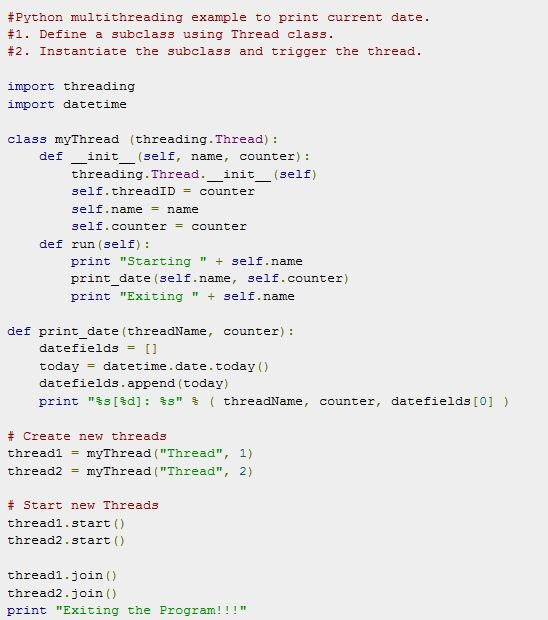
\includegraphics[width=0.75\textwidth]{figures/Thread}}
	\caption{Mengimplementasikan Thread menggunakan Threading}
	\label{Mengimplementasikan Thread menggunakan Threading}
\end{figure}

\chapter{XML Processing}
% Kelas D4 TI 3B Kelompok 3
% Diana Satima Gistivani 1154018
% M. Amran Hakim Siregar 1154106
% Indah Rahmawati 1154070
% Rizky Abdul Ghani Suherli 1154058


\section{Python XML Processing}
  XML adalah bahasa open source portable yang mungkinkan pemrogram mengemangkan aplikasi yang dapat dibaca oleh aplikasi lain, bahasa markup untuk keperluan umum yang disarankan oleh W3C untuk membuat dokumen markup keperluan pertukaran data antar sistem yang beraneka ragam. XML merupakan kelanjutan dari HTML (HyperText Markup Language) yang merupakan bahasa standar untuk melacak Internet.
terlepas dari sistem operasi dan bahasa pengembangnya .
\subsection{Apa itu XML}
  Extensible Markup Languange (XML) adalah bahasa markup seperti HTML atau SGML. 
Ini direkomendasikan oleh World Wide Web Consortium dan tersedia sebagai standar terbuka.
XML sangat berguna untuk mencatat data berukuran kecil dan menengah tanpa memerlukan tulang punggung berbasis SQL  
Pada kenyataanya dalam dunia komputer, sistem komputer dan database mengandung data yang tidak kompatibel satu sama lain. Dengan demikian tidak mungkin terjadinya pertukaran data melalui internet jika terdapat perbedaan sistem operasi dan aplikasi database yang digunakan.
Dengan menggunakan XML untuk pertukaran data, masalah perbedaan platform dan aplikasi tidak perlu diresahkan lagi. karena data yang disimpan pada XML dapat dibaca oleh berbagai macam platform dan aplikasi.

\subsection{Keunggulan dan Kelemahan Python XML Processing}
\subsubsection{Keunggulan Python XML Processing}
\begin{enumerate}
Keunggulan dari python dapat dijabarkan dari faktor-faktor berikut ini :
\item Quality : Python merupakan piranti lunak yang memakai meodologi reusability sehingga komponen-komponen pembangun piranti      lunak mudah digunakan dan diatur.
\item Productivity : penulisan program menggunakan python lebih mudah, karena interpreter menangani source code secara terpisah pada lower-level language.Interpreter menangani tipe deklarasi variabel,manajemen memory dan source code.
\item Portability : program python dapat dieksekusi di berbagai jenis komputer.Dengan demikian proses eksekusi program dapat dilakukan tanpa mengubah source code program.
\item Integration : phyton dirancang untuk dapat berinteraksi dengan aplikasi lain.Dengan demikian,program yang dibangun dengan bahasa pemrograman lain dapat dieksekusi dengan mudah padascript phyton dengan menggunakan function bahasa pemrograman lainnya.
\item Tidak ada tahapan kompilasi dan penyambungan (link) sehingga kecepatan perubahan pada masa pembuatan sistem aplikasi meningkat.
\item Tidak ada deklarasi tipe data yang merumitkan sehingga program menjadi lebih sederhana, singkat, dan fleksible.
\item Manajemen memori otomatis yaitu kumpulan sampah memori sehingga dapat menghindari pencacatan kode.
\item Tipe data dan operasi tingkat tinggi yaitu kecepatan pembuatan sistem aplikasi menggunakan tipe objek yang telah ada.
\item Pemrograman berorientasi objek.
\item Pelekatan dan perluasan dalam C.
\item Terdapat kelas, modul, eksepsi sehingga terdapat dukungan pemrograman skala besar secara modular.
\item Pemuatan dinamis modul C sehingga ekstensi menjadi sederhana dan berkas biner yang kecil
\item Pemuatan kembali secara dinamis modul phyton seperti memodifikasi aplikasi tanpa menghentikannya.
\item Model objek universal kelas Satu.
\item Konstruksi pada saat aplikasi berjalan.
\item Interaktif, dinamis dan alamiah.
\item Akses hingga informasi interpreter.
\item Portabilitas secara luas seperti pemrograman antar platform tanpa ports.
\item Kompilasi untuk portable kode byte sehingga kecepatan eksekusi bertambah dan melindungi kode sumber.
\item Antarmuka terpasang untuk pelayanan keluar seperti perangkat Bantu system, GUI, persistence, database, dll.


\end{enumerate}
 
\subsection {Arsitektur XML dan API}
  Perpustakaan standar Python menyediakan seperangkat antarmuka minimal tapi berguna untuk bekerja dengan XML. Dua API yang paling dasar dan umum digunakan untuk data XML adalah antarmuka SAX dan DOM. 
\subsubsection {System Arsitektur XML}
\begin{enumerate}
Sistem terdiri dari 3 lapisan yaitu :
\item lapisan database :Lapisan ini digunakan untuk menyimpan dokumen XML.Dalam system ini digunakan DBMS SQL Server.SQL
Server mengenalkan tipe data XML.Tipe data ini dapat digunakan dalam definisi tabel untuk mendefinisikan tipe sebuah kolom, tipe variabel dalam kode prosedural Transact-SQL, dan sebagai parameter prosedur.
\item lapisan bahasa query : XML, seperti basisdata relasional, mempunyai bahasa query sendiri yang dioptimasi untuk format data.Berpasangan dengan tipe data xml, hal ini mempercepat dan mengefisienkan penyimpanan dan temukembali data XML.
\item lapisan aplikasi : Lapisan ini merupakan antarmuka menggunakan bahasa Indonesia. Bahasa pemrograman yang digunakan adalah Java.Java menyediakan banyak fasilitas yang memudahkan untuk mengimplementasikan system yang dibuat.

\subsubsection {SAX}
  API sederhana untuk XML (SAX): mendaftarkan panggilan kemali untuk acara yang diminati dan kemudian membiarkan parser berjalan melalui dokumen. Ini berguna bila dokumen berukuran besar atau memiliki keterbatasan memori, ini memparsing file tidak pernah tersimpan dalam memori. Biasanya juga SAX ini dapat di pakai oleh Generator untuk membaca file XML dan pesan SAX ini juga biasa disebut dengan istilah event. SAX akan di kirimkan oleh Generator ke pipeline. SAX atau event ini juga dapat mengirimkan sebuah dokumen atau lampiran yang artinya SAX atau event ini dapat di proses nantinya.
  
\subsubsection {DOM}
  API Document Objek Model (DOM): ini adalah rekomendasi World Wide Web Consortium dimana keseluruhan file dibaca ke memori dan disimpan dalam bentuk hierarkies (tree-based) untuk mewakili semua fitur dokumen XML. 

SAX jelas tidak bisa memproses informasi secepat DOM saat bisa bekerjadengan file besar. Di sisi lain, menggunakan DOM secara eklusifenar-benar dapat membunuh sumber daya, terutama jika digunakan pada banyak file kecil. SAX hanya bisa dibaca sementara DOM mengizinkan perubahan pada file XML. Kedua API yang berbeda ini saling melengkapi satu sama lain, tidak ada alasan mengapa tidak dapat menggunakannya untuk proyek besar. 

Contoh: 
\begin{verbatim}
<collection shelf="New Arrivals"> 
<movie title="Enemy Behind"> 
  <type>War, Thriller</type> 
  <format>DVD</format> 
  <year>2003</year> 
  <rating>PG</rating> 
  <stars>10</stars>
  <description>Talk about a US-Japan war</description> 
</movie> 
<movie title="Transformers"> 
  <type>Anime, Science Fiction</type> 
  <format>DVD</format> 
  <year>1989</year> 
  <rating>R</rating> 
  <stars>8</stars> 
  <description>A schientific fiction</description> 
</movie> 
  <movie title="Trigun"> 
  <type>Anime, Action</type> 
  <format>DVD</format> 
  <episodes>4</episodes>  
  <rating>PG</rating> 
  <stars>10</stars> 
  <description>Vash the Stampede!</description> 
</movie>
<movie title="Ishtar"> 
  <type>Comedy</type> 
  <format>VHS</format> 
  <rating>PG</rating> 
  <stars>2</stars> 
  <description>Viewable boredom</description> 
</movie> 
</collection> 
\end{verbatim}


\subsection{Parsing XML dengan API SAX}
  SAX adalah antarmuka standar untuk parsing XML berbasis event. Parsing XML dengan SAX umumnya mengharuskan untuk membuat dengan subclassing xml.sax.
  ControlHandler menangani tag dan atribut tertentu dari XML. Objek ControlHandler menyediakan metode untuk menangani berbagai aktivitas parsing. Parsing memanggil metode ControlHandler saat memparsing file XML.
  Metode startDocument dan endDocument disebut awal dan akhir setiap elemen. Jika parsing tidak dalam mode namespace, metode startElement (tag attribute) dan endElement (tag) dipanggil. Jika tidak, metode yang sesuai startElemenNS dan endElemenNS dipanggil. 

Berikut ini metode penting untuk memahami sebelum melanjutkan ke materi berikutnya : 
\begin{enumerate}
  \item Metode berikut membuat objek parsing baru dan mengembalikannya. Objek parsing diuat akan menjadi tipe parsing pertama yang ditemukan sistem.
  \item xml.sax.make parser([parser list])
\end{enumerate}

Berikut adalah detail parameternya : 
\begin{enumerate}
  \item Parser list : pilihan argumen yang terdiri dari daftar parsing untuk digunakan yang semuanya harus menerapkan metode {make    parse}.
  \item Metode berikut membuat parsing SAX dan menggunakannya untuk mengurai dokumen. xml.sax.parser(xmlfile, contenthandler[, errorhandler])
\end{enumerate}

Membuat parsing SAX dan mengurai string XML yang ditentukan : 
xml.sax.parsertring(xmlstring,contenthandler[, errorhandler])

Brikut ini adalah detail nama dari parameter : 
\begin{enumerate}
  \item  {XMLstring}  = Nama dari string yang bisa dibaca.
  \item  {ContentHandler} = Menjadi objek ContenHandler.
  \item  {ErrorHandler} = Menjadi objek ErorHandler SAX. 
\end{enumerate}

Contoh : 
\begin{verbatim}
  \#  
  /usr/bin/python
import xml.sax 
class MovieHandler( xml.sax.ContentHandler ): 
~~ def init (self): 
~~~~~ self.CurrentData = "" 
~~~~~ self.type = "" 
~~~~~ self.format = "" 
~~~~~ self.year = "" 
~~~~~ self.rating = "" 
~~~~~ self.stars = "" 
~~~~~ self.description = "" 
~~ \#  Call when an element starts 
~~ def startElement(self, tag, attributes):
~~~~~ self.CurrentData = tag 
~~~~~ if tag == "movie": 
~~~~~~~~ print "*****Movie*****" 
~~~~~~~~ title = attributes["title"] 
~~~~~~~~ print "Title:", title 
~~ \#  Call when an elements ends 
~~ def endElement(self, tag): 
~~~~~ if self.CurrentData == "type":
~~~~~~~~ print "Type:", self.type 
~~~~~ elif self.CurrentData == "format": 
~~~~~~~~ print "Format:", self.format 
~~~~~ elif self.CurrentData == "year": 
~~~~~~~~ print "Year:", self.year 
~~~~~ elif self.CurrentData == "rating": 
~~~~~~~~ print "Rating:", self.rating 
~~~~~ elif self.CurrentData == "stars": 
~~~~~~~~ print "Stars:", self.stars 
~~~~~ elif self.CurrentData == "description": 
~~~~~~~~ print "Description:", self.description 
~~~~~ self.CurrentData = "" 
~~ \#  Call when a character is read 
~~ def characters(self, content): 
~~~~~ if self.CurrentData == "type":
~~~~~~~~ self.type = content 
~~~~~ elif self.CurrentData == "format": 
~~~~~~~~ self.format = content 
~~~~~ elif self.CurrentData == "year": 
~~~~~~~~ self.year = content 
~~~~~ elif self.CurrentData == "rating": 
~~~~~~~~ self.rating = content 
~~~~~ elif self.CurrentData == "stars":
~~~~~~~~ self.stars = content 
~~~~~ elif self.CurrentData == "description": 
~~~~~~~~ self.description = content 
if (name  == " main "): 
~~ \#  create an XMLReader 
~~ parser = xml.sax.make parser() 
~~ \#  turn off namepsaces
~~ parser.setFeature(xml.sax.handler.feature namespaces, 0) 
~~ \#  override the default ContextHandler 
~~ Handler = MovieHandler() 
~~ parser.setContentHandler( Handler )
~~ parser.parse("movies.xml") 
\end{verbatim}

Ini akan menghasilkan hasil sebagai berikut: 
\begin{verbatim}
{*****Movie******} 
{*****Movie*****} 
{Title: Enemy Behind} 
{Type: War, Thriller} 
{Format: DVD} 
{Year: 2003} 
{Rating: PG} 
{Stars: 10} 
{Description: Talk about a US-Japan war}
{*****Movie*****} 
{Title: Transformers} 
{Type: Anime, Science Fiction}
{Format: DVD} 
{Year: 1989} 
{Rating: R}
{Stars: 8} 
{Description: A schientific fiction} 
{*****Movie*****} 
{Title: Trigun} 
{Type: Anime, Action} 
{Format: DVD}
{Rating: PG} 
{Stars: 10} 
{Description: Vash the Stampede!} 
{*****Movie*****} 
{Title: Ishtar}
{Type: Comedy} 
{Format: VHS}
{Rating: PG} 
{Stars: 2} 
\end{verbatim}

\subsection{2.3 Parsing XML dengan API DOM} 
Document Ovject Model (DOM) adalah API lintas bahasa dari World Wide Web Consortium (W3C) untuk mengakses dan memodifikasi dokumen XML.  DOM sangat berguna untuk aplikasi akses acak. SAX hanya memungkinkan melihat satu bit dokumen sekaligus. Jika melihat satu elemen SAX, tidak memiliki akses ke yang lain. Berikut adalah cara termudah untuk memuat dokumen XML dengan cepat dan membuat objek minidom menggunakan modul xml.dom. Objek minidom menyediakan metode parsing sederhana yang dengan cepat memuat pohon DOM dari file XML. \par
Contoh~frase memanggil fungsi  parsing (file [,parsing]) dari objek minidokumen untuk mengurai file XML yang ditunjuk oleh file ke objek pohon DOM.
\begin{enumerate}
\item $  \#  $!/usr/bin/python
from xml.dom.minidom import parse 
import xml.dom.minidom 
\item $  \#  $ Open XML document using minidom parser
DOMTree = xml.dom.minidom.parse("movies.xml") 
collection = DOMTree.documentElement 
if collection.hasAttribute("shelf"): 
print "Root element :  $  \%  $s"  $  \%  $ collection.getAttribute("shelf") 
\item $  \#  $ Get all the movies in the collection 
movies = collection.getElementsByTagName("movie") 
\item $  \#  $ Print detail of each movie. 
for movie in movies: 
print "*****Movie*****" 
if movie.hasAttribute("title"): 
print "Title:  $  \%  $s"  $  \%  $ movie.getAttribute("title") 
type = movie.getElementsByTagName('type')[0] 
print "Type:  $  \%  $s"  $  \%  $ type.childNodes[0].data 
format = movie.getElementsByTagName('format')[0] 
print "Format:  $  \%  $s"  $  \%  $ format.childNodes[0].data 
rating = movie.getElementsByTagName('rating')[0] 
print "Rating:  $  \%  $s"  $  \%  $ rating.childNodes[0].data 
description = movie.getElementsByTagName('description')[0] 
print "Description:  $  \%  $s"  $  \%  $ description.childNodes[0].data 
Ini akan menghasilkan hasil sebagai berikut : 
Root element : New Arrivals 
*****Movie***** 
Title: Enemy Behind 
Type: War, Thriller 
Format: DVD 
Rating: PG 
Description: Talk about a US-Japan war 
*****Movie***** 
Title: Transformers 
Type: Anime, Science Fiction 
Format: DVD 
Rating: R 
Description: A schientific fiction 
*****Movie***** 
Title: Trigun 
Type: Anime, Action 
Format: DVD 
Rating: PG 
Description: Vash the Stampede! 
*****Movie***** 
Title: Ishtar 
Type: Comedy 
Format: VHS 
Rating: PG
Description: Viewable boredom 
\end{enumerate}

\subsection{Membangun Parsing Document XML menggunakan Python} 
Python mendukung untuk bekerja dengan berbagai bentuk markup data terstruktur. Selain mengurai xml.etree. \textit{ElementTree} mendukung pembuatan dokumen XML yang terbentuk dengan baik dari objek elemen yang dibangun dalam aplikasi. Kelas elemen digunakakan saat sebuah dokumen diurai untuk mengetahui bagaimana menghasilkan bentuk serial dari isinya kemudian dapat ditulis ke sebuah file.  
Untuk membuat instance elemeb gunakan fungsi elemen contructor dan \textit{SubElemen()} pabrik. 
Import xml.etree.ElementTree as xml \par
\vspace{12pt}
\noindent 
{\fontsize{10pt}{10pt}\selectfont filename =  $ " $/home/abc/Desktop/test $  \_  $xml.xml $ " $} \par
\noindent 
{\fontsize{10pt}{10pt}\selectfont toot = xml.Element( $ " $Users $ " $)} \par
\noindent 
{\fontsize{10pt}{10pt}\selectfont userelement = xml.Element( $ " $user $ " $)} \par
\noindent 
{\fontsize{10pt}{10pt}\selectfont root.append(userelement)} \par
\noindent 
\vspace{10pt}
\noindent 
Bila menjalankan ini, akan menghasilkan sebagai berikut : \par
\noindent 
{\fontsize{10pt}{10pt}\selectfont <Users>} \par
\noindent 
{\fontsize{10pt}{10pt}\selectfont  \hspace*{0.5in} <user>} \par
\noindent 
{\fontsize{10pt}{10pt}\selectfont  \hspace*{0.5in} <user>} \par
\noindent 
{\fontsize{10pt}{10pt}\selectfont </Users>} \par
\vspace{10pt}
\vspace{10pt}
\vspace{10pt}
\noindent 
Tambahkan anak-anak pegguna \par
\vspace{10pt}
\noindent 
{\fontsize{10pt}{10pt}\selectfont Uid = xml.SubElement(userelement,  $ " $uid $ " $)} \par
\noindent 
{\fontsize{10pt}{10pt}\selectfont Uid.text =  $ " $1 $ " $} \par
\vspace{10pt}
\noindent 
{\fontsize{10pt}{10pt}\selectfont FirstName = xml.SubElement(userelement,  $ " $FirstName $ " $)} \par
\noindent 
{\fontsize{10pt}{10pt}\selectfont FirstName.text =  $ " $testuser $ " $} \par
\vspace{10pt}
\noindent 
{\fontsize{10pt}{10pt}\selectfont LastName = xml.SubElement(userelement,  $ " $LastName $ " $} \par
\noindent 
{\fontsize{10pt}{10pt}\selectfont LastName.text =  $ " $testuser $ " $} \par
\vspace{10pt}
\noindent 
{\fontsize{10pt}{10pt}\selectfont Email = xml.SubElement(userelement,  $ " $Email $ " $)} \par
\noindent 
{\fontsize{10pt}{10pt}\selectfont Email.text = {mailto:testuser@test.com}{testuser@test.com}
} \par
\vspace{10pt}
\noindent 
{\fontsize{10pt}{10pt}\selectfont state = xml.SubElement(userelemet,  $ " $state $ " $)} \par
\noindent 
{\fontsize{10pt}{10pt}\selectfont state.text =  $ " $xyz $ " $} \par
\vspace{10pt}
\noindent 
{\fontsize{10pt}{10pt}\selectfont location = xml.SubElement(userelement,  $ " $location)} \par
\noindent 
{\fontsize{10pt}{10pt}\selectfont location.text = abc} \par
\vspace{10pt}
\noindent 
{\fontsize{10pt}{10pt}\selectfont tree = xml.ElementTree(root)} \par
\noindent 
{\fontsize{10pt}{10pt}\selectfont with open(filename,  $ " $w $ " $) as fh:} \par
\noindent 
{\fontsize{10pt}{10pt}\selectfont tree.write(fh)} \par
\vspace{10pt}
\noindent 
 \hspace*{0.5in} Pertama buat elemen root dengan mengunakan fungsi \textit{ElementTree}. Kemudian membuat elemen pegguna dan menambahkannya ke root. Selanjutnya membuat \textit{SubElement }dengan melewatkan elemen pengguna (userelement) ke \textit{SubElemen} beserta namanya seperto  $ " $FirstName $ " $. Kemudian untuk setiap \textit{SubElement} tetapkan properti teks untuk memberi nilai. Di akhir, membuat \textit{ElementTree} dan menggunakannya untuk menulis XML ke file. \par
\noindent 
 \hspace*{0.5in} Jika menjalankan ini akan menjadi sebagai berikut : \par
\noindent 
 {\fontsize{10pt}{10pt}\selectfont <users>} \par
\noindent 
{\fontsize{10pt}{10pt}\selectfont  \hspace*{0.5in} <user>} \par
\noindent 
{\fontsize{10pt}{10pt}\selectfont  \hspace*{0.5in}  \hspace*{0.5in} <uid>1</uid>} \par
\noindent 
{\fontsize{10pt}{10pt}\selectfont  \hspace*{0.5in}  \hspace*{0.5in} <FirstName>testuser</FirstName>} \par
\noindent 
{\fontsize{10pt}{10pt}\selectfont  \hspace*{0.5in}  \hspace*{0.5in} <LastName>testuser</LastName>} \par
\noindent 
{\fontsize{10pt}{10pt}\selectfont  \hspace*{0.5in}  \hspace*{0.5in} <state>xyz</state>} \par
\noindent 
{\fontsize{10pt}{10pt}\selectfont  \hspace*{0.5in}  \hspace*{0.5in} <location>abc</location>} \par
\noindent 
{\fontsize{10pt}{10pt}\selectfont  \hspace*{0.5in} </user>} \par
\noindent 
{\fontsize{10pt}{10pt}\selectfont </Users>} \par
\vspace{10pt}
\noindent 
Parsing XML Documen : \par
\vspace{12pt}
\noindent 
{\fontsize{10pt}{10pt}\selectfont import xml.etree.ElementTree as ET} \par
\noindent 
{\fontsize{10pt}{10pt}\selectfont tree = ET.parse(‘Your $  \_  $XML $  \_  $file $  \_  $path’)} \par
\noindent 
{\fontsize{10pt}{10pt}\selectfont root = tree.getroot()} \par
\noindent 
{\fontsize{10pt}{10pt}\selectfont 

 %%%%%%%%%%%%  Start New Page here %%%%%%%%%%%%%%


\newpage

}\vspace{10pt}
\vspace{10pt}
\noindent 
Disini \textit{getroot()} akan mengembalikan elemen dari dokumen XML \par
\vspace{10pt}
\noindent 
{\fontsize{10pt}{10pt}\selectfont <Users version= $ " $1.0 $ " $ languange= $ " $SPA $ " $>} \par
\noindent 
{\fontsize{10pt}{10pt}\selectfont  \hspace*{0.5in} <user>} \par
\noindent 
{\fontsize{10pt}{10pt}\selectfont  \hspace*{0.5in}  \hspace*{0.5in} <uid>1</uid>} \par
\noindent 
{\fontsize{10pt}{10pt}\selectfont  \hspace*{0.5in}  \hspace*{0.5in} <FirstName>testuser</FirstName>} \par
\noindent 
{\fontsize{10pt}{10pt}\selectfont  \hspace*{0.5in}  \hspace*{0.5in} <LastName>testuser</LastName>} \par
\noindent 
{\fontsize{10pt}{10pt}\selectfont  \hspace*{0.5in}  \hspace*{0.5in} <Email>testuser@tes.com/Email>} \par
\noindent 
{\fontsize{10pt}{10pt}\selectfont  \hspace*{0.5in}  \hspace*{0.5in} <state>xyz</state>} \par
\noindent 
{\fontsize{10pt}{10pt}\selectfont  \hspace*{0.5in}  \hspace*{0.5in} <location>abc</location>} \par
\noindent 
{\fontsize{10pt}{10pt}\selectfont  \hspace*{0.5in} </user>} \par
\noindent 
{\fontsize{10pt}{10pt}\selectfont </Users>} \par
\vspace{12pt}


\chapter{GUI Programming}
\documentclass [12pt,a4paper,notitlepage,oneside,bahasa]{article}
\usepackage[left=3.00 cm, right=2.00 cm, bottom=2.00 cm, top=3.00 cm]{geometry}
\begin{document}
\title{\textbf GUI Programming}
\maketitle

Python menyediakan berbagai pilihan untuk mengembangkan antarmuka pengguna grafis (GUIs). 
Berikut dibawah ini merupakan berbagai pilihan yang disediakan oleh Python :
\begin{itemize}
\item Tkinter \par
Tkinter merupakan standar bahasa python yang ditetapkan untuk membangun suatu antarmuka pengguna grafik (GUI). 
\item wxPython \par
wxPython adalah toolkit antarmuka pengguna grafis (GUI) yang digunakan dalam skripsi ini dan ini adalah pembungkus untuk toolkit wxWidgets.
\item Jpython \par
Port Python untuk java yang memberikan Python script akses tanpa batas ke perpustakaan kelas java pada mesin lokal \par
\end{itemize}
\vspace{12pt}
\noindent 
\section{\textbf Tkinter Pemrograman}
Tkinter adalah perpustakaan GUI standar untuk Python. Python bila dikombinasikan dengan Tkinter menyediakan cara yang amat mudah dan cepat untuk membuat aplikasi GUI. Tkinter menyediakan antarmuka yang berorientasi objek yang kuat untuk toolkit Tk GUI.
 \hspace*{0.5in} Membuat aplikasi GUI menggunakan Tkinter adalah tugas yang mudah. Yang diperlukan adalah melakukan langkah-langkah sebagai berikut : 
\begin{enumerate} 
	\item Mengimpor Tkinter modul 
	\item Buat jendela utama aplikasi GUI
	\item Tambahkan satu atau lebih dari widget tersebut diatas ke aplikasi GUI
	\item Masukkan acara loop utama untuk mengambil tindakan terhadap setiap peristiwa dipicu oleh pengguna
\end{enumerate}

 %%%%%%%%%%%%  Start New Page here %%%%%%%%%%%%%%


\newpage

\vspace{12pt}
\vspace{12pt}
\noindent 
Contoh : 
\begin{verbatim}
#!/usr/bin/python 
import Tkinter 
top = Tkinter.Tk()
# Code to add widgets will go here...
top.mainloop()
\end{verbatim}

\section{\textbf Tkinter Widget} \par
\noindent 
 \hspace*{0.5in} Tkinter menyediakan berbagai kontrol seperti tombol, label dan kotak teks yang digunakan dalam aplikasi GUI. 
 Kontrol ini biasanya disebut widget.
\noindent 
 \hspace*{0.5in} Saat ini ada 15 jenis widget di Tkinter. berikut adalah contoh widget serta penjelasan singkat pada tabel ini:


 %%%%%%%%%%%%  Table No:1 Here %%%%%%%%%%%%%%


\begin{table}[h]
	\caption{Ukuran}
		\begin{center}
		\begin{tabular}{|c|c|}
			\hline
			Operator & Penjelasan \\
			\hline
			Button & Menampilkan tombol dalam aplikasi\\
			Canvas & Menggambar bentuk seperti garis, oval, poligon dan persegi panjang dalam aplikasi\\
			Checkbutton & Menampilkan sejumlah pilihan sebagai kotak centang. Pengguna dapat memilih beberapa pilihan pada suatu waktu
			Entry & Menampilkan bidang garis teks tunggal untuk menerima nilai-nilai dari pengguna\\
			Frame & Wadah untuk mengatur widget lainnya\\
			Label & Memberikan keterangan garis single untuk widget lainnya. Hal ini berisi gambar\\
			Listbox & Menyediakan daftar pilihan kepada pengguna\\
			Menubutton & Menampilkan menu dalam aplikasi\\
			Menu & Memberikan berbagai perintah untuk pengguna. Perintah-perintah ini terkandung di dalam MenuButton\\
			Message & Menampilkan bidang teks multiline untuk menerima nilai-nilai dari pengguna\\
			RadioButton & Menampilkan sejumah pilihan sebagai tombol radio. Pengguna dapat memilih hanya satu pilihan pada suatu waktu\\
			Scale & Menyediakan widget slide\\
			Scrollbar & Menambah kemampuan bergulir ke berbagai widget seperti kotak daftar\\
			Text & Menampilka teks dalam beberapa garis\\
			Toplevel & Menyediakan wajah jendela terpisah\\
			PanedWindow & Wadah yang mengandung sejumlah panel disusun horizontal atau vertikal\\
			LabelFrame & Wadah widget sederhana. Bertindak sebagai spacer atau wajah untuk layout jendela kompleks\\
			TkMessageBox & Menampilkan kotak pesan dalam aplikasi\\
			Spinbox & Memilih sejumlah tetap nilai-nilai&\\
		\hline
		\end{tabular}
		\end{center}
	\begin{tablenotes}
	\end{tablenotes}
\end{table}

	


 %%%%%%%%%%%%  Table No:1 Ends Here %%%%%%%%%%%%%%


\vspace{12pt}
subsection{Atribut Tkinter}
\noindent 
 \hspace*{0.5in} Beberapa atribut umum sebagai ukuran, warna dan font ditentukan. Berikut adalah beberapa atribut standar :
\noindent 
\begin{enumerate}
\item Ukuran 
Berbagai panjang, lebar, dan dimensi lain dari widget digambarkan dalam banyak unit yang berbeda seperti 
\item Jika menetapkan dimensi ke integer diasumsikan dalam piksel 
\item Menentukan unit dengan menentukan dimensi untuk string yang berisi sejumlah diikuti oleh :
\end{itemize}
 


 %%%%%%%%%%%%  Table No:2 Here %%%%%%%%%%%%%%


\begin{table}[ht]
	\caption{Ukuran}
	\bein{center}
	\begin{tabular}{|c|c|}
		\hline
		Karakter&  Penjelasan \cr
		\hline
		c&Sentimeter\\
		i&Inci\\
		m&Milimeter\\
		p&Poin printer\\
		\hline
	\end{tabular}
	\end{center}
	\begin{tablenotes}
	\end{tablenotes}
\end{table}


 %%%%%%%%%%%%  Table No:2 Ends Here %%%%%%%%%%%%%%

 
 \hspace*{0.5in} \vspace{12pt}
 subsection{Panjang Tkinter}
 \hspace*{0.5in} Tkinter mengungkapkan panjang sebagai integer jumlah piksel. Berikut ini adalah daftar pilihan panjang umum:
\noindent 
\begin{itemize}
	\item borderwidth
	Lebar batas yang memberikan tampilan tiga dimensi untuk widget
	\item highlightthickness
	Lebar puncak persegi panjang ketika widget memiliki fokus
 	\item padX padY
	Ruang tambahan widget dari manajer tata letak luar minimum widget perlu menampilkan isinya di x dan y arah
	\item selectborderwidth
	Lebar perbatasan tiga dimensi disekitar dipilih item widget
	\item wraplength \par
	Panjang garis maksimum untuk widget yang melakukan kata membungkus
	\item height
	Tinggi diinginkan widget
	\item underline
	Indeks karakter untuk menggarisawahi dalam teks widget 
	\item width
	\item Lebar diinginkan widget
\end{itemize}
 
\noindent 
subsection{Warna Tkinter}
\noindent 
Tkinter memiliki warna dengan string. Ada dua cara umum untuk menentukan sebuah warna di Tkiter, yaitu : \par
\noindent 
\begin{itemize}
	\item Menggunakan string menentukan proporsi merah, hijau dan biru didigit heksadesimal. Misalnya  `` \#ffff '' putih,  ``  \#000000 '' hitam dan  ``\#000fff000 '' hijau.
\noindent 
	\item Menggunakan lokal standar nama warna . warna-warna ``white'', ``black'',  ``green'' dan  ``magenta'' akan selalu tersedia.
\end{itemize}

\vspace{12pt}
Pilihan warna umum :
\noindent 
\begin{itemize}
	\item activebackground \par
	Warna latar berlakang untuk widget ketika widget aktif \par
	\noindent 
	\item activeforeground \par
	Warna depan untuk widget ketika widget aktif \par
	\noindent 
	\item background \par
	Merepresentasikan sebagai \textit{bg} \par
	\noindent 
	\item disableforeground \par
	Warna depan untuk widget ketika widget dinonaktifkan \par
	\noindent 
	\item foreground \par
	Merepresentasikan fg \par
	\noindent 
	\item highlightbackground \par
	Warna latar belakang dari daerah puncak ketika widget memiliki fokus \par
	\noindent 
	\item hightlightcolor \par
	Warna depan dari wilayah puncak ketika widget memiliki fokus \par
	\noindent 
	\item selectbackground \par
	Warna latar belakang untuk item yang dipilih dari widget \par
	\noindent 
	\item selectforeground \par
	Warna depan untuk item yang dipilih dari widget \par
	\noindent 
	\item Font \par
	\noindent 
	Sebagai tupel yang elemen pertama adalah keluarga font diikuti dengan string yang berisi satu atau lebih gaya pengubah tebal,miring, garis bawah dan overstrike. 
	end{itemize}
	\noindent 
Contoh : \par
	\begin{itemize}
		\noindent
		\item ( ``Helvetica'', ``16 '') untuk 16 \- point Helvetica biasa \par
		\noindent 
		\item ( ``Times'', ``24 '',``beranimiring'') untuk 24 \- point kali miring tebal
	\end{itemize}
 		\par
\vspace{12pt}
Dapat membuat  ``font object'' dengan mengimpor modul tkFont dan menggunakan kelas konstruktor font nya : \par
Import tkFont \par
Font = tkFont.Font (option, ....) \par
\vspace{12pt}
Berikut adalah daftar pilihan : \par
\noindent 
\begin{itemize}
	\item Family \par
	Font nama keluarga sebagai string \par
	\noindent 
	\item Size \par
	Font tinggi sebagai integer dalam poin \par
	\noindent 
	\item Weight \par
	Bold untuk teal, normal untuk berat badan secara teratur \par
	\noindent 
	\item Slant \par
	Italic untuk miring, roman untuk unstlanted \par
	\noindent 
	\item Underline \par
	1 untuk teks yang digarisbawahi, 0 untuk normal \par
	\noindent 
	\item Overstrike \par
	1 untuk teks telak, 0 untuk normal \par
	Jika berjalan di bawah X window system, dapat menggunakan salah satu nama font X. Sebagai contoh, font bernama  \verb|"-*lucidatypewriter-medium-r-*-*-*-140-*-*-*"| adalah favorit fixed-width font penulis untuk digunakan pada layar. \par
	\noindent 
	\item Jangkar \par
	\noindent 
	Jangkar digunakan untuk mendefinisikan mana teks diposisikan relatif terhadap titik acuan. Berikut adalah daftar kemungkinan konstanta yang dapat digunakan :
	\noindent
	\begin{itemize}
		\item NW  
		\item N
		\item NE
		\item W
		\item TENGAH
		\item E
		\item SW
		\item S
		\item SE
	\end{itemize}
\end{itemize}
 \par
\vspace{12pt}
Jika menggunakan tengah sebagai jangkar tek, tek akan ditengahkan horizontal dan vertikal disekitar titik referensi. \par
Jangkar NW akan posisi teks sehingga titik referensi bertepatan dengan laut sudut kotak berisi teks \par
Jangakr W akan pusat teks secara vertikal disekitar satu titik referensi dengan tepi kiri kotak teks yang melewati titik itu dan sebagainya. \par
Jika membuat widget kecil didalam bingkai besar dan menggunakan jangkar = SE pilihan, widget akan ditempatkan disudut kanan bawah gambar. Jika menggunakan anchor = N sebaliknya widget akan dipusatkan disepanjang tepi atas. \par
\noindent 

subsection{Gaya relief}

Widget mengacu pada efek 3-D simulasi terbaru disekitar bagian luar widget. Berikut adalah daftar konstanta yang mungkin dapat digunakan untuk atribut:
\begin{itemize}
	\item Datar
	\item Dibesarkan
	\item Cekung
	\item Alur
	\item Punggung bukit
\end{itemize}


\vspace{12pt}
Contoh : \par
{\fontsize{10pt}{10pt}\selectfont From Tkinter import *} \par
{\fontsize{10pt}{10pt}\selectfont Import Tkinter} \par
\vspace{10pt}
{\fontsize{10pt}{10pt}\selectfont top = Tkinter.Tk()} \par
{\fontsize{10pt}{10pt}\selectfont B1 = Tkinter.Button(top, text= $ " $FLAT $ " $, relief=FLAT)} \par
{\fontsize{10pt}{10pt}\selectfont B2 = Tkinter.Button(top, text= $ " $RAISED $ " $, relief=RAISED)} \par
{\fontsize{10pt}{10pt}\selectfont B3 =Tkinter.Button(top, text= $ " $SUNKEN $ " $, relief=SUNKEN)} \par
{\fontsize{10pt}{10pt}\selectfont B4=Tkinter.Button(top, text= $ " $GROOVE $ " $, relief=GROOVE)} \par
{\fontsize{10pt}{10pt}\selectfont B5=Tkinter.Button(top, text= $ " $RIDGE $ " $, relief=RIDGE)} \par
\vspace{10pt}
{\fontsize{10pt}{10pt}\selectfont B1.pack()} \par
{\fontsize{10pt}{10pt}\selectfont B2.pack()} \par
{\fontsize{10pt}{10pt}\selectfont B3.pack()} \par
{\fontsize{10pt}{10pt}\selectfont B4.pack()} \par
{\fontsize{10pt}{10pt}\selectfont B5.pack()} \par
{\fontsize{10pt}{10pt}\selectfont top.mainloop()} \par
\noindent 
Britmaps \par
\noindent 
Ada beberapa jenis bitmap yang tersedia, diantaranya: \par
\noindent 
\begin{itemize}
\item Kesalahan \par
\noindent 
\item Gray75 \par
\noindent 
\item Gray50 \par
\noindent 
\item Gray12 \par
\noindent 
\item Jam Pasir \par
\noindent 
\item Info \par
\noindent 
\item Questhead \par
\noindent 
\item Perantanyaan  \par
\noindent 
\item Peringatan\end{itemize}
 \par
\vspace{12pt}
Contoh: \par
{\fontsize{10pt}{10pt}\selectfont From Tkinter import *} \par
{\fontsize{10pt}{10pt}\selectfont Import Tkinter} \par
\vspace{10pt}
{\fontsize{10pt}{10pt}\selectfont Top = Tkinter.Tk()} \par
\vspace{10pt}
{\fontsize{10pt}{10pt}\selectfont B1 = Tkinter.Button(top, text = $ " $error $ " $, relief=RAISED,  $  \setminus  $ bitmap= $ " $error $ " $)} \par
{\fontsize{10pt}{10pt}\selectfont B2 = Tkinter.Button(top, text = $ " $hourglass $ " $, relief=RAISED,  $  \setminus  $ bitmap= $ " $hourglass $ " $)} \par
{\fontsize{10pt}{10pt}\selectfont B3 = Tkinter.Button(top, text = $ " $info $ " $, relief=RAISED,  $  \setminus  $ bitmap= $ " $info $ " $)} \par
{\fontsize{10pt}{10pt}\selectfont B4 = Tkinter.Button(top, text = $ " $question $ " $, relief=RAISED,  $  \setminus  $ bitmap= $ " $question $ " $)} \par
{\fontsize{10pt}{10pt}\selectfont B5 = Tkinter.Button(top, text = $ " $warning $ " $, relief=RAISED,  $  \setminus  $ bitmap= $ " $warning $ " $)} \par
\vspace{10pt}
{\fontsize{10pt}{10pt}\selectfont B1.pack()} \par
{\fontsize{10pt}{10pt}\selectfont B2.pack()} \par
{\fontsize{10pt}{10pt}\selectfont B3.pack()} \par
{\fontsize{10pt}{10pt}\selectfont B4.pack()} \par
{\fontsize{10pt}{10pt}\selectfont B5.pack()} \par
{\fontsize{10pt}{10pt}\selectfont top.mainloop()} \par
\noindent 
Kursor \par
\noindent 
Berikut daftar menarik : \par
\noindent 
\begin{itemize}
\item Panah \par
\noindent 
\item Lingkaran \par
\noindent 
\item Jam \par
\noindent 
\item Menyebrang \par
\noindent 
\item Dotbox \par
\noindent 
\item Bertukar \par
\noindent 
\item Fluer \par
\noindent 
\item Jantung \par
\noindent 
\item Manusia \par
\noindent 
\item Tikus \par
\noindent 
\item Bajak laut \par
\noindent 
\item Tamah \par
\noindent 
\item Antar jemput \par
\noindent 
\item Perekat \par
\noindent 
\item Laba-laba \par
\noindent 
\item Kaleng semprot \par
\noindent 
\item Bintang \par
\noindent 
\item Target \par
\noindent 
\item Tcross \par
\noindent 
\item Melakukan perjalanan \par
\noindent 
\item Menonton\end{itemize}
 \par
\vspace{12pt}
Contoh : \par
{\fontsize{10pt}{10pt}\selectfont From Tkinter import *} \par
{\fontsize{10pt}{10pt}\selectfont Import Tkinter} \par
\vspace{10pt}
{\fontsize{10pt}{10pt}\selectfont Top = Tkinter.Tk()} \par
\vspace{10pt}
{\fontsize{10pt}{10pt}\selectfont B1 = Tkinter.Button(top, text = $ " $circle $ " $, relief=RAISED,  $  \setminus  $ bitmap= $ " $circle $ " $)} \par
{\fontsize{10pt}{10pt}\selectfont B2 = Tkinter.Button(top, text = $ " $plus $ " $, relief=RAISED,  $  \setminus  $ bitmap= $ " $plus $ " $)} \par
\vspace{10pt}
{\fontsize{10pt}{10pt}\selectfont B1.pack()} \par
{\fontsize{10pt}{10pt}\selectfont B2.pack()} \par
{\fontsize{10pt}{10pt}\selectfont top.mainloop()} \par
\vspace{10pt}
\noindent 
\textbf{3.3 Manajemen Geometri} \par
\noindent 
 \hspace*{0.5in} Semua widget tkinter memiliki akses ke metode manajemen geometri tertentu, yang memiliki tujuan menggorganisir widget diseluruh wilayah widget induk. Tkinter mengekspos kelas manager geometri berikut : \par
\noindent 
\begin{itemize}
\item Metode the \textit{pack()} \par
\noindent 
Manajer geometri ini mengatur widget diblok sebelum menempatkan mereka di widget induk \par
\noindent 
\item Metode the \textit{grid()} \par
\noindent 
Manajer geometri ini mengatur widget dalam struktur tabel seperti di widget induk \par
\noindent 
\item Metode the  \textit{place()}\end{itemize} \par
\noindent 
Manajer geometri ini mengatur widget dengan menempatkan dalam posisi tertentu dalam widget induk \par
\vspace{12pt}
\noindent 
\textbf{3.4 Manfaat Tkinter} \par
Tkinter sangat sederhana. Berikut manfaat Tkinter dibandingkan GUI toolkit : \par
\noindent 
\begin{itemize}
\item 
Tkinter terdiri dari sejumlah modul.  (Tkinter)\vspace{\baselineskip}
Antarmuka Tk terletak di modul biner
bernama _tkinter (ini adalah tkinter di versi sebelumnya). Modul ini berisi lowlevel
antarmuka ke Tk, dan tidak boleh digunakan langsung oleh pemrogram aplikasi. ini
biasanya shared library (atau DLL), tapi mungkin dalam beberapa kasus secara statis terkait dengan
Penerjemah Python. \par
\noindent
\item Tkinter mudah diakses oleh siapa saja. (Accessibilty)\vspace{\baselineskip}
Tkinter merupakan toolkit yang ringan dan satu-satunya solusi GUI yang paling sederhana untuk Python sampai saat ini. Cukup menuliskan 
beberapa baris kode Python untuk membuat aplikasi GUI sederhana dengan Tkinter. Untuk menambahkan komponen baru pada Tkinter, dapat 
membuatnya dalam kode Python atau menambahkan paket ekstensi seperti Pmw, Tix, atau ttk. \par
\noindent 
\item widget root tk (widget root tk)\vspace{\baselineskip}
Untuk menginisialisasi Tkinter, kita harus membuat widget root Tk. Ini adalah jendela biasa, dengan
judul bar dan hiasan lainnya yang disediakan oleh window manager Anda. Anda seharusnya saja
buat satu widget root untuk setiap program, dan itu harus dibuat sebelum widget lainnya. \par
\noindent 
\item Tkinter mudah digunakan di semua platform (Portability)\vspace{\baselineskip}
Sebuah program Python yang dibangun menggunakan Tkinter dapat berjalan dengan baik di semua platform sistem operasi seperti Microsoft 
Windows, Linux, dan Macintosh. Dan dari segi tampilan window, akan terlihat sama dengan standar platform yang digunakan. \par
\noindent 
\item Tkinter selalu tersedia di Python (Availability)\vspace{\baselineskip}
Tkinter merupakan modul standar pada pustaka Python. Sebagian besar paket instalasi Python sudah langsung berisi Tkinter. Khusus untuk 
beberapa distro Linux, perlu menambahkan paket Tkinter secara terpisah. Pada Windows, bisa langsung menggunakan Tkinter sesaat setelah 
menginstal paket instalasi Python. \par
\noindent 
\item handles bagus di gunakan di Python (Handles)\vspace{\baselineskip}
item kandles merupakan nilai integer yang digunakan untuk mengidentifikasi item tertentu pada kanvas. Tkinter secara otomatis menugaskan 
pegangan baru ke setiap item baru yang dibuat di atas kanvas. Item Handles dapat di lewatkan ke berbagai metode kanvas baik sebagai 
bilangan bulat atau sebagai string. Tag adalah nama simbolis yang dilekatkan pada item. Tag adalah string biasa, dan bisa berisi apa 
saja kecuali spasi (asalkan tidak sesuai dengan item pegangan). \par
\noindent 
\item Modul Tkinter menyediakan kelas yang sesuai dengan berbagai jenis widget di Tk (Module)\vspace{\baselineskip}
dan sejumlah mixin dan kelas pembantu lainnya (mixin adalah kelas yang dirancang untuk menjadi
dikombinasikan dengan kelas lain menggunakan multiple inheritance). Bila Anda menggunakan Tkinter, Anda
jangan pernah mengakses kelas mixin secara langsung. \par
\noindent 
\item Dokumentasi Tkinter sangat LUAR BIASA (Documentation)\vspace{\baselineskip}
Python (plus Tkinter) ini bersifat open-source, maka banyak sekali komunitas-komunitas yng membahas Python dan Tkinter dan bisa belajar dan bertanya langsung dengan para ahli.\end{itemize}
 \par
\vspace{12pt}
\vspace{12pt}

\end{document}


\chapter{Futher Expression}
\begin{center}{\fontsize{14pt}{14pt}\selectfont \textbf{FURTHER EXPRESSION} \\}\end{center} 
\vspace{14pt}

 \hspace*{0.5in} Stiap kode yang dituliskan menggunakan bahasa yang dikompilasi seperti C, C++ atau Java dapat diintegrasikan ke skrip Python lainnya. Kode ini diagnggap sebagai ektensi. 

 \hspace*{0.5in} Modul ekstensi Python tidak lebih dari sekedar perpustakaan C biasa. Pada mesin Unix, perpustakaan ini biasanya diakhiri dengan .so (untuk objek bersama). Pada mesin windows, biasanya melihat .dll (untuk perpusatkaan yang terhubung secara dinamis).  
\vspace{12pt}

\textbf{4.1 Pra-Persyaratan untuk Menulis Ekstensi} 

 \hspace*{0.5in} Untuk memulai ektensi, memerlukan file header Python. Pada mesin Unix, biasanya memerlukan instalasi paket khusus pengembang seperti python 2-5. 

 \hspace*{0.5in} Pengguna window mendapatkan header ini sebagai bagian dari paket saat menggunakan pemasang Python biner. 

 \hspace*{0.5in} Harus memiliki pengetahuan yang baik tentang C atau C++ untuk menulis ekstensi Python menggunakan pemrograman C. 
 
 \hspace*{0.5in} Untuk melihat modul ekstensi Python, perlu mengelompokkan kode menjadi empat bagian : 

\begin{itemize}
\item File header Python h 

\item Fungsi C yang ingin ditampilkan sebagai antarmuka dari modul 
 
\item Sebuah tabel memetakan nama-nama fungsi saat pengembang Python melihat ke fungsi C didalam modul ekstensi 

\item Fungsi inilisasi\end{itemize}
 
\vspace{12pt}
Perlu menyertakan file header Python.h di file sumber C memberi akses ke API Python internal digunakan untuk menghitung modul ke penerjamah. 
Menyertakan header Python.h sebelum header lain yang mungkin dibutuhkan. Mengikuti termasuk dengan fungsi yang ingin dipanggil dari Python. 
Tanda tangan penerapan C fungsi selalu mengambil salah satu dari tiga bentuk berikut : 

{\fontsize{10pt}{10pt}\selectfont static PyObject *MyFunction( PyObject *self, PyObject *args );} 
 
\vspace{10pt}
 
{\fontsize{10pt}{10pt}\selectfont static PyObject *MyFunctionWithKeywords(PyObject *self,} 

{\fontsize{10pt}{10pt}\selectfont ~~~~~~~~~~~~~~~~~~~~~~~~~~~~ PyObject *args,} 

{\fontsize{10pt}{10pt}\selectfont ~~~~~~~~~~~~~~~~~~~~~~~~~~~~ PyObject *kw);} 

\vspace{10pt}

{\fontsize{10pt}{10pt}\selectfont static PyObject *MyFunctionWithNoArgs( PyObject *self );} 
\vspace{12pt}

 \hspace*{0.5in} Masing-masing deklarasi seelumnya mengembalikan objek Python. Tidak ada yang namanya fungsi void dengan Python seperti ada di C. Jika ingin fungsi mengembalikan nilai, Python. Header Python mendefinisikan makro. Py $  \_  $Return $  \_  $None yang melakukan ini. 

 \hspace*{0.5in} Nama-nama fungsi C bisa menjadi apapun yang disuka karena tidak pernah diluar modul ekstensi mendefinisikan sebagai statis. 

 \hspace*{0.5in} Fungi Cbiasanya diberi nama dengan menggabnungkan modul dan fungsi Python bersama-sama yang ditunjukan disini : 


static PyObject *\textit{module $  \_  $func}(PyObject *self, PyObject *args)  $  \{  $ 

~~ /* Do your stuff here. */ 

~~ Py $  \_  $RETURN $  \_  $NONE; 

 $  \}  $ 
\vspace{12pt}
\vspace{12pt}
 
 \hspace*{0.5in} Ini adalah fungsi Python yang disebut func didalam modul-modul. Memasukkan petunjuk ke fungsi C ke dalam tabel metode untuk modul yang biasanya muncul selanjutnya dikode sumber tael pemetaan metode. 

 \hspace*{0.5in} Tabel metode ini adalah susunan sederhana dari struktur PyMethodSef. Struktur itu terlihat seperti ini : 

struct PyMethodDef  $  \{  $ 
 
~~ char *ml $  \_  $name; 
 
~~ PyCFunction ml $  \_  $meth; 

~~ int ml $  \_  $flags; 
 
~~ char *ml $  \_  $doc; 

 $  \}  $; 
\vspace{12pt}

Inilai uraian anggota struktur ini : 

\begin{itemize}
\item Ml $  \_  $name 
Nama fungsi yang digunakan penafsir Python saat digunakan dalam program Python 

\item Ml $  \_  $meth 
Menjadi alamaat ke fungsi yang memiliki salah satu tanda tangan yang dijelaskan dalam penelusuran sebelumnya 

\item Ml $  \_  $flags 
Memberitahu penafsir yang mana dari tiga tanda tangan yang digunakan ml $  \_  $meth. Bendera ini biasanya mmiliki nilai meth $  \_  $varargs. Bendera ini dapat digandakan dengan or’ed dengan meth $  \_  $keywords jika ingin memiarkan argumen kata kunci masuk ke fungsi. Ini juga bisa memiliki nilai meth $  \_  $noargs yang menunjukan bahwa tidak ingin menerima argumen apa pun. 

\item Ml $  \_  $doc 
Ini adalah docstring untuk fungsi yang bisa jadi NULL jika tidak ingin menulisnya. 
\vspace{12pt}
\vspace{12pt}

 \hspace*{0.5in} Tabel ini perlu diakhiri dengan sentinel yang terdiri dari NULL dan 0 untuk anggota yang sesuai. 
\vspace{12pt}

Contoh: 

static PyMethodDef \textit{module} $  \_  $methods[] =  $  \{  $ 

~~  $  \{  $ "\textit{func}", (PyCFunction)\textit{module $  \_  $func}, METH $  \_  $NOARGS, NULL  $  \}  $, 

~~  $  \{  $ NULL, NULL, 0, NULL  $  \}  $ 

 $  \}  $; 
\vspace{12pt}

 \hspace*{0.5in} Bagian terakhir dari modul ekstensi adalah fungsi inialisasi. Fungsi ini dipanggil oleh juru bahasa Python saat modul diisikan. Hal ini diperlukan agar fungsi diberi nama intiModule dimana modul adalah nama modul. 

 \hspace*{0.5in} Fungsi inialisasi perlu diekspor dari perpustakaan yang akan dibangun. Header Python mendefinisikan PyMODINIT $  \_  $Func untuk memasukkan mantra yang sesuai agar terjadi pada lingkungan tertentu tempat menyuusun. Yang harus dilakukan adalah mengunakan saat menentukan fungsinya. 

 \hspace*{0.5in} Fungsi inialisasi C umumnya memiliki strktur keseluruhan berikut : 

PyMODINIT $  \_  $FUNC init\textit{Module}()  $  \{  $ 

~~ Py $  \_  $InitModule3(\textit{func}, \textit{module} $  \_  $methods, "docstring..."); 

 $  \}  $ 
\vspace{12pt}

Berikut adalah penjelasan fugsi Py $  \_  $IntiModule : 

\item Func  

Ini adalah fungsi yang akan diekspor 

\item Module 

Ini adalah nama tabel pemetaan yang didefinisikan diatas 

\item Docstring\end{itemize}
 

Ini adalah komentar yang ingin diberikan diekstensi 
\vspace{12pt}

 \hspace*{0.5in} Menempatkan ini semua bersama-sama terlihat sebagai berikut : 

 $  \#  $include <Python.h>
\vspace{12pt}

static PyObject *\textit{module $  \_  $func}(PyObject *self, PyObject *args)  $  \{  $ 

~~ /* Do your stuff here. */ 

~~ Py $  \_  $RETURN $  \_  $NONE; 

 $  \}  $ 
\vspace{12pt}

static PyMethodDef \textit{module} $  \_  $methods[] =  $  \{  $ 

~~  $  \{  $ "\textit{func}", (PyCFunction)\textit{module $  \_  $func}, METH $  \_  $NOARGS, NULL  $  \}  $, 
 
~~  $  \{  $ NULL, NULL, 0, NULL  $  \}  $ 

 $  \}  $; 
\vspace{12pt}

PyMODINIT $  \_  $FUNC init\textit{Module}()  $  \{  $ 
 
~~ Py $  \_  $InitModule3(\textit{func}, \textit{module} $  \_  $methods, "docstring..."); 

 $  \}  $ 
\vspace{12pt}
\vspace{12pt}

Contoh : 
 
 $  \#  $include <Python.h> 
\vspace{12pt}
 
static PyObject* helloworld(PyObject* self) 

 $  \{  $ 
 
~~~ return Py $  \_  $BuildValue("s", "Hello, Python extensions!!"); 

 $  \}  $ 
\vspace{12pt}
 
static char helloworld $  \_  $docs[] = 
static PyMethodDef helloworld $  \_  $funcs[] =  $  \{  $ 

~~~  $  \{  $"helloworld", (PyCFunction)helloworld,  

~~~~ METH $  \_  $NOARGS, helloworld $  \_  $docs $  \}  $, 

~~~  $  \{  $NULL $  \}  $
 
 $  \}  $; 
\vspace{12pt}

void inithelloworld(void) 
 
 $  \{  $ 

~~~ Py $  \_  $InitModule3("helloworld", helloworld $  \_  $funcs, 

~~~~~~~~~~~~~~~~~~ "Extension module example!"); 
 
 $  \}  $ 
\vspace{12pt}
\vspace{12pt}
 
 \hspace*{0.5in} Disini fungsi Py $  \_  $BuildValue digunakan untuk membangun nilai Python.  
\vspace{12pt}
\vspace{12pt}
 
\textbf{4.2 Membangun dan Menginstal Ekstensi} 
\vspace{12pt}
\vspace{12pt}

 \hspace*{0.5in} Distutils paket membuatnya sangat mudah mendistribusikan modul Python, baik Python murni dan modul ekstensi dengan cara standar. Modul didistribusikan dalam bentuk sumber dan dibangun dan diinstal melalui skrip setup yang iasa disebut seup.py sebagai berikut : 
 
from distutils.core import setup, Extension \par
~~~~~ ext $  \_  $modules=[Extension('helloworld', ['hello.c'])]). 
\vspace{12pt}

 \hspace*{0.5in} Sekarang gunakan perintah berikut yang aka melalakukan semua kompilasi dan langkah penghubunh yang diperlukan dengan perintah dan bendera penyusun dan penghubung yang benar dan menyalin perpustakaan dinamis yang dihasilkan ke dalam direktori yang sesuai . 
\vspace{12pt}
 
Contoh : 
 
 $  \$  $ python setup.py install 
\vspace{12pt}
 
 \hspace*{0.5in} Pada sistem berbasis Unix kemungkinan besar perlu menjalankan perintah ini sebagai root agar meminta izin untuk menulis ke direktori paket situs. Ini biasanya tidak menjadi masalah pada window. 
Setelah~menginstal ekstensi, akan dapat mengimpor dan memanggil ekstensi tersebut di skrip Python  sebagai berikut : 

 $  \#  $!/usr/bin/python 
 
import helloworld 
\vspace{12pt}

print helloworld.helloworld() 
\vspace{14pt}
 
Ini~akan menghasilkan hasil sebagai berikut  : 

Hello, Python extensions!! 
\vspace{12pt}
Seperti kemungkinan besar ingin mendefinisikan fungsi yang menerima argumen, dapat menggunakan salah satu tanda tangan lain untuk fungsi C. Sebagai contoh, fungsi berikut yang menerima beberapa parameter akan didefinisikan seperti ini : 

static PyObject *\textit{module $  \_  $func}(PyObject *self, PyObject *args)  $  \{  $ 

~~ /* Parse args and do something interesting here. */ 

~~ Py $  \_  $RETURN $  \_  $NONE; 

 $  \}  $ 
\vspace{12pt}
Tabel metode yang berisi entri untuk fungsi baru akan terlihat seperti ini : 

static PyMethodDef \textit{module} $  \_  $methods[] =  $  \{  $ 

~~  $  \{  $ "\textit{func}", (PyCFunction)\textit{module $  \_  $func}, METH $  \_  $NOARGS, NULL  $  \}  $, 

~~  $  \{  $ "\textit{func}", \textit{module $  \_  $func}, METH $  \_  $VARARGS, NULL  $  \}  $, 

~~  $  \{  $ NULL, NULL, 0, NULL  $  \}  $ 

 $  \}  $; 
\vspace{12pt}
Menggunakan fungsi API PyArg $  \_  $ParseTuple untuk mengekstrak argumen dari satu pointer PyObject yang dikirimkan ke fungsi C. Argumen pertama untuk PyArg $  \_  $ParseTuple adalah args argumen. Ini adalah objek yang akan parsing. Argumen kedua adalah string format yang menggambarkan argumen saat mengharapkannya muncul. Setiap argumen diwakili oleh satu atau lebih karakter dalam format string sebagai berikut : 

static PyObject *\textit{module $  \_  $func}(PyObject *self, PyObject *args)  $  \{  $ 

~~ int i;

~~ double d; 

~~ char *s; 
\vspace{12pt}

~~ if (!PyArg $  \_  $ParseTuple(args, "ids",  $  \&  $i,  $  \&  $d,  $  \&  $s))  $  \{  $ 

~~~~~ return NULL; 

~~  $  \}  $ 

~~  

~~ /* Do something interesting here. */ 

~~ Py $  \_  $RETURN $  \_  $NONE; 

 $  \}  $ 
\vspace{12pt}
Mengkompilasi versi baru dari modul dan mengimpornya memungkinkan untuk memanggil fungsi baru dengan sejumlah argumen dari jenis apa pun : 

module.func(1, s="three", d=2.0) 

module.func(i=1, d=2.0, s="three") 

module.func(s="three", d=2.0, i=1) 
\vspace{12pt}
\vspace{12pt}
\vspace{12pt}
\vspace{12pt}

 \hspace*{0.5in} Berikut adalah tanda tangan standar untuk fungsi PyArg $  \_  $ParseTuple: 
 
int PyArg $  \_  $ParseTuple(PyObject* tuple,char* format,...) 
\vspace{12pt}

 \hspace*{0.5in} Fungsi ini mengembalikan 0 untuk kesalahan, dan nilai tidak sama dengan 0 untuk kesuksesan. Tuple adalah PyObject * yang merupakan argumen kedua dari fungsi C. Format berikut adalah string C yang menggambarkan argumen wajib dan opsional.\vspace{\baselineskip}
~~~~~~ Berikut adalah daftar kode format untuk fungsi PyArg $  \_  $ParseTuple: 


 %%%%%%%%%%%%  Table No:1 Here %%%%%%%%%%%%%%


\begin{table}[ht]
	\caption{Ukuran}
	\begin{tabular*}{\textwidth}{@{\extracolsep{\fill}}lcc}
		\hline
		Karakter&  Penjelasan \cr
		\hline
		c&Sentimeter&\cr
		i&Inci&\cr
		m&Milimeter&\cr
		p&Poin printer\cr
		\hline
	\end{tabular*}
	\begin{tablenotes}
	\end{tablenotes}
\end{table}

 %%%%%%%%%%%%  Table No:1 Ends Here %%%%%%%%%%%%%%


\vspace{12pt}
\vspace{14pt}
Py $  \_  $BuildValue~mengambil format string seperti PyArg $  \_  $ParseTuple. Alih-alih menyampaikan alamat nilai yang sedang  bangun, melewati nilai sebenarnya. Berikut adalah contoh yang menunjukkan bagaimana menerapkan fungsi tambah : 

static PyObject *foo $  \_  $add(PyObject *self, PyObject *args)  $  \{  $ 

~~ int a; 

~~ int b; 
\vspace{12pt}

~~ if (!PyArg $  \_  $ParseTuple(args, "ii",  $  \&  $a,  $  \&  $b))  $  \{  $ 

~~~~~ return NULL;

~~  $  \}  $ 

~~ return Py $  \_  $BuildValue("i", a + b); 

 $  \}  $ 
\vspace{14pt}
Ini adalah apa yang akan terlihat seperti jika diimplementasikan dengan Python : 

def add(a, b):

~~ return (a + b) 
\vspace{16pt}
Mengembalikan dua nilai dari fungsi sebagai berikut, ini akan dipicu menggunakan daftar dengan Python :

static PyObject *foo $  \_  $add $  \_  $subtract(PyObject *self, PyObject *args)  $  \{  $ 

~~ int a; 

~~ int b; 
\vspace{12pt}

~~ if (!PyArg $  \_  $ParseTuple(args, "ii",  $  \&  $a,  $  \&  $b))  $  \{  $ 

~~~~~ return NULL; 

~~  $  \}  $ 

~~ return Py $  \_  $BuildValue("ii", a + b, a - b); 

 $  \}  $ 
\vspace{16pt}
Ini adalah apa yang akan terlihat seperti jika diimplementasikan dengan Python : 

def add $  \_  $subtract(a, b): 

~~ return (a + b, a - b) 
\vspace{14pt}
Berikut~adalah tanda tangan standar untuk fungsi Py $  \_  $BuildValue  : 

PyObject* Py $  \_  $BuildValue(char* format,...) 
\vspace{14pt}
Format berikut adalah string C yang menggambarkan objek Python untuk dibangun. Argumentasi berikut Py $  \_  $BuildValue adalah nilai C dari mana hasilnya dibuat. Hasil PyObject * adalah referensi baru.  
Berikut daftar tabel string kode yang umum digunakan, yang nol atau lebihnya digabungkan ke dalam format string : 


 %%%%%%%%%%%%  Table No:2 Here %%%%%%%%%%%%%%


\begin{table}[ht]
	\caption{Ukuran}
	\begin{tabular*}{\textwidth}{@{\extracolsep{\fill}}lcc}
		\hline
		Code& C Type&  Meaning\cr
		\hline
		c&char&String Python dengan panjang 1 menjadi huruf C.\cr
		d&double&Pelampung Python menjadi C ganda.\cr
		f&float&Pelampung Python menjadi pelampung C.\cr
		i&int&Int Python menjadi int int\cr
		l&long&Sebuah int Python menjadi panjang C.\cr
		L&long long&Sebuah int Python menjadi C panjang panjang\cr
		O&PyObject*&Gets non-NULL meminjam referensi ke argumen Python\cr
		s&char*&Python string tanpa nulls tertanam ke C char *\cr
		s&char*+int&Setiap string Python ke alamat dan panjang C\cr
		t&char*+int&Read-only penyangga segmen tunggal ke alamat C dan panjangnya\cr
		U&PyUNICODE*&Python Unicode tanpa nulls tertanam ke C\cr
		u&PPyUNICODE*int+&Setiap alamat dan panjang Python Unicode C\cr
		w&char*+int&Membaca / menulis penyangga segmen tunggal ke alamat dan panjang C\cr
		Z&char*&Seperti s, juga menerima None (set C char * ke NULL).\cr
		z&char*+int&Seperti s, juga menerima None set C char * ke NULL\cr
		(...)&Poin printer&Urutan Python diperlakukan sebagai satu argumen per item.\cr
		|&as per ...&Argumen berikut bersifat opsional.\cr
		:&&Format akhir, diikuti dengan nama fungsi untuk pesan error.\cr
		;&&Format akhir, diikuti oleh seluruh pesan kesalahan teks.\cr				
		\hline
	\end{tabular*}
	\begin{tablenotes}
	\end{tablenotes}
\end{table}


 %%%%%%%%%%%%  Table No:2 Ends Here %%%%%%%%%%%%%%


\vspace{12pt}
Kode  $  \{  $... $  \}  $ membangun kamus dari sejumlah nilai C, kunci dan nilai bergantian. Misalnya, Py $  \_  $BuildValue (" $  \{  $issi $  \}  $", 23, "zig", "zag", 42) mengembalikan kamus seperti  $  \{  $23: 'zig', 'zag': 42 $  \}  $ Python. 
Setiap blok memori yang dialokasikan dengan malloc () pada akhirnya harus dikembalikan ke genangan memori yang tersedia dengan satu panggilan untuk membebaskan (). Penting untuk menelepon gratis () pada waktu yang tepat. Jika alamat blok dilupakan tapi gratis () tidak dipanggil untuk itu, memori yang ditempatinya tidak dapat digunakan kembali sampai program berakhir. Ini disebut kebocoran memori. Di sisi lain, jika sebuah program memanggil gratis () untuk satu blok dan kemudian terus menggunakan blok tersebut, itu menciptakan konflik dengan penggunaan ulang blok melalui panggilan malloc () yang lain. Ini disebut dengan menggunakan memori yang dibebaskan. Ini memiliki konsekuensi buruk yang sama seperti merujuk pada data yang tidak diinisiasi - dump inti, hasil yang salah, crash misterius. 
Karena Python membuat penggunaan malloc () dan gratis (), dibutuhkan strategi untuk menghindari kebocoran memori dan juga penggunaan memori yang bebas. Metode yang dipilih disebut penghitungan referensi. Prinsipnya sederhana: setiap objek berisi sebuah counter, yang bertambah saat referensi ke objek disimpan di suatu tempat, dan yang dikurangi saat referensi itu dihapus. Saat counter mencapai nol, referensi terakhir ke objek telah dihapus dan objeknya dibebaskan. 



\begin{references}{3.}
\bibitem{kilby}J. S. Kilby,
``Invention of the Integrated Circuit,'' {\it IEEE Trans. Electron Devices,}
{\bf ED-23,} 648 (1976).

\bibitem{hamming}R. W. Hamming,
                 {\it Numerical Methods for Scientists and 
                 Engineers}, Chapter N-1, McGraw-Hill, 
                 New York, 1962.

\bibitem{Hu}J. Lee, K. Mayaram, and C. Hu, ``A Theoretical
               Study of Gate/Drain Offset in LDD MOSFETs''
                     {\it IEEE Electron Device Lett.,} {\bf EDL-7}(3). 152 
                     (1986).

\bibitem{beren}A. Berenbaum, 
B. W. Colbry, D.R. Ditzel, R. D Freeman, and 
K.J. O'Connor, ``A Pipelined 32b Microprocessor with 13 kb of Cache Memory,''
{it Int. Solid State Circuit Conf., Dig. Tech. Pap.,} p. 34 (1987).
\end{references}


\begin{references}{Ham62}
\bibitem[Kil76]{kilb}J. S. Kilby,
``Invention of the Integrated Circuit,'' {\it IEEE Trans. Electron Devices,}
{\bf ED-23,} 648 (1976).

\bibitem[Ham62]{hamm}R. W. Hamming,
                 {\it Numerical Methods for Scientists and 
                 Engineers}, Chapter N-1, McGraw-Hill, 
                 New York, 1962.

\bibitem[Hu86]{lee}J. Lee, K. Mayaram, and C. Hu, ``A Theoretical
               Study of Gate/Drain Offset in LDD MOSFETs''
                     {\it IEEE Electron Device Lett.,} {\bf EDL-7}(3). 152 
                     (1986).

\bibitem[Ber87]{berm}A. Berenbaum, 
B. W. Colbry, D.R. Ditzel, R. D Freeman, and 
K.J. O'Connor, ``A Pipelined 32b Microprocessor with 13 kb of Cache Memory,''
{it Int. Solid State Circuit Conf., Dig. Tech. Pap.,} p. 34 (1987).

\end{references}



%%%%%%%%%%%%%%%
%%  The default LaTeX Index
%%  Don't need to add any commands before \begin{document}
\printindex

%%%% Making an index
%% 
%% 1. Make index entries, don't leave any spaces so that they
%% will be sorted correctly.
%% 
%% \index{term}
%% \index{term!subterm}
%% \index{term!subterm!subsubterm}
%% 
%% 2. Run LaTeX several times to produce <filename>.idx
%% 
%% 3. On command line, type  makeindx <filename> which
%% will produce <filename>.ind 
%% 
%% 4. Type \printindex to make the index appear in your book.
%% 
%% 5. If you would like to edit <filename>.ind 
%% you may do so. See docs.pdf for more information.
%% 
%%%%%%%%%%%%%%%%%%%%%%%%%%%%%%

%%%%%%%%%%%%%% Making Multiple Indices %%%%%%%%%%%%%%%%
%% 1. 
%% \usepackage{multind}
%% \makeindex{book}
%% \makeindex{authors}
%% \begin{document}
%% 
%% 2.
%% % add index terms to your book, ie,
%% \index{book}{A term to go to the topic index}
%% \index{authors}{Put this author in the author index}
%% 
%% \index{book}{Cows}
%% \index{book}{Cows!Jersey}
%% \index{book}{Cows!Jersey!Brown}
%% 
%% \index{author}{Douglas Adams}
%% \index{author}{Boethius}
%% \index{author}{Mark Twain}
%% 
%% 3. On command line type 
%% makeindex topic 
%% makeindex authors
%% 
%% 4.
%% this is a Wiley command to make the indices print:
%% \multiprintindex{book}{Topic index}
%% \multiprintindex{authors}{Author index}

\end{document}

